\documentclass[11pt,a4paper]{article}
\usepackage[utf8]{inputenc}
\usepackage[T1]{fontenc}
\usepackage[margin=0.75in]{geometry}
\usepackage{amsmath,amssymb,amsfonts}
\usepackage{graphicx}
\usepackage{booktabs}
\usepackage{tabularx}
\usepackage{xltabular}
\usepackage{hyperref}
\usepackage{listings}
\usepackage{xcolor}
\usepackage{float}
\usepackage{enumitem}

\newcolumntype{C}{>{\centering\arraybackslash}X}
\newcolumntype{L}{>{\raggedright\arraybackslash}X}
\newcolumntype{R}{>{\raggedleft\arraybackslash}X}

\graphicspath{{../plots/}{./plots/}{plots/}}

\hypersetup{
    colorlinks=true,
    linkcolor=blue,
    urlcolor=blue,
    citecolor=blue
}

\lstset{
    basicstyle=\ttfamily\small,
    breaklines=true,
    backgroundcolor=\color{gray!10},
    frame=single,
    framerule=0.5pt,
    rulecolor=\color{gray!30},
    keywordstyle=\color{blue}\bfseries,
    commentstyle=\color{green!60!black},
    stringstyle=\color{orange}
}

\title{\textbf{Advanced Database Management Systems (ADBMS)\\[0.5em] \Large Assignment 0 \& Assignment 1: Histogram Analysis Report}}
\author{\textbf{ADBMS Coursework Submission}}
\date{\today}

\begin{document}
\maketitle
\tableofcontents
\newpage
\section{Advanced Database Management Systems (ADBMS)}
\subsection{Assignment 0 \& Assignment 1: Histogram Analysis Report}

\hrule


\section{Assignment 0}

\subsection{Setup}
\begin{itemize}
\item \textbf{CPU Model \& Specification}: 13th Gen Intel(R) Core(TM) i3-1315U (6 cores, 8 threads)
\item \textbf{RAM Capacity}: 14 GiB
\item \textbf{HDD / Storage Capacity}: 456 GiB NVMe SSD
\item \textbf{Operating System}: Ubuntu 26.04 LTS
\item \textbf{PostgreSQL Engine Version}: \texttt{PostgreSQL 18.6 (Ubuntu 18.6-0ubuntu0.26.04.1) on x86\_64-pc-linux-gnu, compiled by gcc (Ubuntu 15.2.0-16ubuntu1) 15.2.0, 64-bit}
\end{itemize}

\subsection{Database}
\begin{itemize}
\item \textbf{Database Name}: Join Order Benchmark (2013 Snapshot)
\item \textbf{Total Tables}: 21
\item \textbf{Total Relational Tuples}: 74,190,187
\end{itemize}

\subsubsection{Table Cardinalities \& Primary Keys}

{\begingroup
\small
\setlength{\tabcolsep}{5pt}
\begin{xltabular}{\textwidth}{l | C | C}
\toprule
\textbf{Table Name} & \textbf{Primary Key Column} & \textbf{Cardinality (\texttt{count(*)})} \\
\midrule
\endfirsthead
\toprule
\textbf{Table Name} & \textbf{Primary Key Column} & \textbf{Cardinality (\texttt{count(*)})} \\
\midrule
\endfirsthead
\endhead
\bottomrule
\endfoot
\bottomrule
\endlastfoot
\texttt{aka\_name} & \texttt{id} & 901,343 \\
\texttt{aka\_title} & \texttt{id} & 361,472 \\
\texttt{cast\_info} & \texttt{id} & 36,244,344 \\
\texttt{char\_name} & \texttt{id} & 3,140,339 \\
\texttt{comp\_cast\_type} & \texttt{id} & 4 \\
\texttt{company\_name} & \texttt{id} & 234,997 \\
\texttt{company\_type} & \texttt{id} & 4 \\
\texttt{complete\_cast} & \texttt{id} & 135,086 \\
\texttt{info\_type} & \texttt{id} & 113 \\
\texttt{keyword} & \texttt{id} & 134,170 \\
\texttt{kind\_type} & \texttt{id} & 7 \\
\texttt{link\_type} & \texttt{id} & 18 \\
\texttt{movie\_companies} & \texttt{id} & 2,609,129 \\
\texttt{movie\_info} & \texttt{id} & 14,835,720 \\
\texttt{movie\_info\_idx} & \texttt{id} & 1,380,035 \\
\texttt{movie\_keyword} & \texttt{id} & 4,523,930 \\
\texttt{movie\_link} & \texttt{id} & 29,997 \\
\texttt{name} & \texttt{id} & 4,167,491 \\
\texttt{person\_info} & \texttt{id} & 2,963,664 \\
\texttt{role\_type} & \texttt{id} & 12 \\
\texttt{title} & \texttt{id} & 2,528,312 \\
\end{xltabular}
\endgroup}


\hrule


\section{Assignment 1: Histogram}

\subsection{Q1. Histogram Analysis for \texttt{id} and \texttt{title} Columns of \texttt{title} Table}

\subsubsection{1. Corresponding SQL Query}
to see what all colums needed form `pg\_stats'

\begin{lstlisting}[language=sql]
\d pg_stats;
\end{lstlisting}

to see histogram boundary values and other relevent  stored in \texttt{pg\_stats}:

\begin{lstlisting}[language=sql]
SELECT 
    attname, 
    null_frac, 
    n_distinct, 
    most_common_vals, 
    most_common_freqs, 
    histogram_bounds 
FROM pg_stats
WHERE tablename = 'title' 
  AND attname IN ('id', 'title');
\end{lstlisting}


\subsubsection{2. Kind of Histogram}
PSQL uses an Equi Depth Histogram combined with a Most Common Values list. In an equidepth histogram, all buckets contain approximately the same number of rows ($approx N / B$), while bucket boundaries vary in width according to data distribution


\subsubsection{3. Number of Buckets}
\begin{itemize}
\item Column \texttt{id}: \textbf{100 buckets} (101 bucket boundary values)
\item Column \texttt{title}: \textbf{100 buckets} (101 bucket boundary values)
\item extra -  to see the defualt number of buckets
\end{itemize}
\begin{lstlisting}[language=sql]
SHOW default_statistics_target;
\end{lstlisting}


\subsubsection{4. How Textual Attribute \texttt{title} is Put into Histogram}
textual attribute “title” is put into histogram as:

1. sorting the text strings in lexicographical order like bannana and apple will be apple, bannana after sorting

2. Sampling string values from the table like table title has around 2.5M rows , it will only sample around 30K

3. Encoding initial string prefix bytes into floating-point numbers in $[0.0, 1.0]$ range for quantitative interpolation like laptop will be broken to lap with l = 108, a=97, p=112 then by 256 as between 0 and 1 , lap will be around 0.42 , we can then see where a key belongs between two keeys

4. Selecting quantile boundary string values at equal percentile intervals to form the 100 equi-depth bucket boundaries stored in \texttt{pg\_stats.histogram\_bounds}.


\subsubsection{5. Exact Bucket Boundaries List (From \texttt{pg\_stats})}

\paragraph{A. Column \texttt{id} Bucket Boundaries (101 values, 100 buckets)}
{\begingroup
\small
\setlength{\tabcolsep}{5pt}
\begin{xltabular}{\textwidth}{l | C | C}
\toprule
\textbf{Bucket Index} & \textbf{Boundary Value (\texttt{id})} & \textbf{Bucket Interval} \\
\midrule
\endfirsthead
\toprule
\textbf{Bucket Index} & \textbf{Boundary Value (\texttt{id})} & \textbf{Bucket Interval} \\
\midrule
\endfirsthead
\endhead
\bottomrule
\endfoot
\bottomrule
\endlastfoot
B000 (Start) & \texttt{59} & Start of table data \\
B001 & \texttt{23714} & Bucket 1: [\texttt{59} - \texttt{23714}] \\
B002 & \texttt{48149} & Bucket 2: [\texttt{23714} - \texttt{48149}] \\
B003 & \texttt{72817} & Bucket 3: [\texttt{48149} - \texttt{72817}] \\
B004 & \texttt{95729} & Bucket 4: [\texttt{72817} - \texttt{95729}] \\
B005 & \texttt{121074} & Bucket 5: [\texttt{95729} - \texttt{121074}] \\
B006 & \texttt{144977} & Bucket 6: [\texttt{121074} - \texttt{144977}] \\
B007 & \texttt{169683} & Bucket 7: [\texttt{144977} - \texttt{169683}] \\
B008 & \texttt{196989} & Bucket 8: [\texttt{169683} - \texttt{196989}] \\
B009 & \texttt{223879} & Bucket 9: [\texttt{196989} - \texttt{223879}] \\
B010 & \texttt{248693} & Bucket 10: [\texttt{223879} - \texttt{248693}] \\
B011 & \texttt{273990} & Bucket 11: [\texttt{248693} - \texttt{273990}] \\
B012 & \texttt{298306} & Bucket 12: [\texttt{273990} - \texttt{298306}] \\
B013 & \texttt{324285} & Bucket 13: [\texttt{298306} - \texttt{324285}] \\
B014 & \texttt{351943} & Bucket 14: [\texttt{324285} - \texttt{351943}] \\
B015 & \texttt{377665} & Bucket 15: [\texttt{351943} - \texttt{377665}] \\
B016 & \texttt{402562} & Bucket 16: [\texttt{377665} - \texttt{402562}] \\
B017 & \texttt{427165} & Bucket 17: [\texttt{402562} - \texttt{427165}] \\
B018 & \texttt{450041} & Bucket 18: [\texttt{427165} - \texttt{450041}] \\
B019 & \texttt{476541} & Bucket 19: [\texttt{450041} - \texttt{476541}] \\
B020 & \texttt{504001} & Bucket 20: [\texttt{476541} - \texttt{504001}] \\
B021 & \texttt{530892} & Bucket 21: [\texttt{504001} - \texttt{530892}] \\
B022 & \texttt{554936} & Bucket 22: [\texttt{530892} - \texttt{554936}] \\
B023 & \texttt{579382} & Bucket 23: [\texttt{554936} - \texttt{579382}] \\
B024 & \texttt{605662} & Bucket 24: [\texttt{579382} - \texttt{605662}] \\
B025 & \texttt{635724} & Bucket 25: [\texttt{605662} - \texttt{635724}] \\
B026 & \texttt{660098} & Bucket 26: [\texttt{635724} - \texttt{660098}] \\
B027 & \texttt{685503} & Bucket 27: [\texttt{660098} - \texttt{685503}] \\
B028 & \texttt{711514} & Bucket 28: [\texttt{685503} - \texttt{711514}] \\
B029 & \texttt{738280} & Bucket 29: [\texttt{711514} - \texttt{738280}] \\
B030 & \texttt{761949} & Bucket 30: [\texttt{738280} - \texttt{761949}] \\
B031 & \texttt{786224} & Bucket 31: [\texttt{761949} - \texttt{786224}] \\
B032 & \texttt{813130} & Bucket 32: [\texttt{786224} - \texttt{813130}] \\
B033 & \texttt{839650} & Bucket 33: [\texttt{813130} - \texttt{839650}] \\
B034 & \texttt{865127} & Bucket 34: [\texttt{839650} - \texttt{865127}] \\
B035 & \texttt{890846} & Bucket 35: [\texttt{865127} - \texttt{890846}] \\
B036 & \texttt{916422} & Bucket 36: [\texttt{890846} - \texttt{916422}] \\
B037 & \texttt{942321} & Bucket 37: [\texttt{916422} - \texttt{942321}] \\
B038 & \texttt{966414} & Bucket 38: [\texttt{942321} - \texttt{966414}] \\
B039 & \texttt{992402} & Bucket 39: [\texttt{966414} - \texttt{992402}] \\
B040 & \texttt{1018536} & Bucket 40: [\texttt{992402} - \texttt{1018536}] \\
B041 & \texttt{1042654} & Bucket 41: [\texttt{1018536} - \texttt{1042654}] \\
B042 & \texttt{1067771} & Bucket 42: [\texttt{1042654} - \texttt{1067771}] \\
B043 & \texttt{1095109} & Bucket 43: [\texttt{1067771} - \texttt{1095109}] \\
B044 & \texttt{1118783} & Bucket 44: [\texttt{1095109} - \texttt{1118783}] \\
B045 & \texttt{1143773} & Bucket 45: [\texttt{1118783} - \texttt{1143773}] \\
B046 & \texttt{1166042} & Bucket 46: [\texttt{1143773} - \texttt{1166042}] \\
B047 & \texttt{1189434} & Bucket 47: [\texttt{1166042} - \texttt{1189434}] \\
B048 & \texttt{1214917} & Bucket 48: [\texttt{1189434} - \texttt{1214917}] \\
B049 & \texttt{1238698} & Bucket 49: [\texttt{1214917} - \texttt{1238698}] \\
B050 & \texttt{1265284} & Bucket 50: [\texttt{1238698} - \texttt{1265284}] \\
B051 & \texttt{1289292} & Bucket 51: [\texttt{1265284} - \texttt{1289292}] \\
B052 & \texttt{1316374} & Bucket 52: [\texttt{1289292} - \texttt{1316374}] \\
B053 & \texttt{1341809} & Bucket 53: [\texttt{1316374} - \texttt{1341809}] \\
B054 & \texttt{1368155} & Bucket 54: [\texttt{1341809} - \texttt{1368155}] \\
B055 & \texttt{1390856} & Bucket 55: [\texttt{1368155} - \texttt{1390856}] \\
B056 & \texttt{1415494} & Bucket 56: [\texttt{1390856} - \texttt{1415494}] \\
B057 & \texttt{1440189} & Bucket 57: [\texttt{1415494} - \texttt{1440189}] \\
B058 & \texttt{1470241} & Bucket 58: [\texttt{1440189} - \texttt{1470241}] \\
B059 & \texttt{1495070} & Bucket 59: [\texttt{1470241} - \texttt{1495070}] \\
B060 & \texttt{1521219} & Bucket 60: [\texttt{1495070} - \texttt{1521219}] \\
B061 & \texttt{1548321} & Bucket 61: [\texttt{1521219} - \texttt{1548321}] \\
B062 & \texttt{1573875} & Bucket 62: [\texttt{1548321} - \texttt{1573875}] \\
B063 & \texttt{1601158} & Bucket 63: [\texttt{1573875} - \texttt{1601158}] \\
B064 & \texttt{1626461} & Bucket 64: [\texttt{1601158} - \texttt{1626461}] \\
B065 & \texttt{1651255} & Bucket 65: [\texttt{1626461} - \texttt{1651255}] \\
B066 & \texttt{1676102} & Bucket 66: [\texttt{1651255} - \texttt{1676102}] \\
B067 & \texttt{1699392} & Bucket 67: [\texttt{1676102} - \texttt{1699392}] \\
B068 & \texttt{1723296} & Bucket 68: [\texttt{1699392} - \texttt{1723296}] \\
B069 & \texttt{1748662} & Bucket 69: [\texttt{1723296} - \texttt{1748662}] \\
B070 & \texttt{1775889} & Bucket 70: [\texttt{1748662} - \texttt{1775889}] \\
B071 & \texttt{1803023} & Bucket 71: [\texttt{1775889} - \texttt{1803023}] \\
B072 & \texttt{1829223} & Bucket 72: [\texttt{1803023} - \texttt{1829223}] \\
B073 & \texttt{1857858} & Bucket 73: [\texttt{1829223} - \texttt{1857858}] \\
B074 & \texttt{1881086} & Bucket 74: [\texttt{1857858} - \texttt{1881086}] \\
B075 & \texttt{1903361} & Bucket 75: [\texttt{1881086} - \texttt{1903361}] \\
B076 & \texttt{1927998} & Bucket 76: [\texttt{1903361} - \texttt{1927998}] \\
B077 & \texttt{1951928} & Bucket 77: [\texttt{1927998} - \texttt{1951928}] \\
B078 & \texttt{1976104} & Bucket 78: [\texttt{1951928} - \texttt{1976104}] \\
B079 & \texttt{1999905} & Bucket 79: [\texttt{1976104} - \texttt{1999905}] \\
B080 & \texttt{2024316} & Bucket 80: [\texttt{1999905} - \texttt{2024316}] \\
B081 & \texttt{2049744} & Bucket 81: [\texttt{2024316} - \texttt{2049744}] \\
B082 & \texttt{2074672} & Bucket 82: [\texttt{2049744} - \texttt{2074672}] \\
B083 & \texttt{2100120} & Bucket 83: [\texttt{2074672} - \texttt{2100120}] \\
B084 & \texttt{2124364} & Bucket 84: [\texttt{2100120} - \texttt{2124364}] \\
B085 & \texttt{2150361} & Bucket 85: [\texttt{2124364} - \texttt{2150361}] \\
B086 & \texttt{2173917} & Bucket 86: [\texttt{2150361} - \texttt{2173917}] \\
B087 & \texttt{2197820} & Bucket 87: [\texttt{2173917} - \texttt{2197820}] \\
B088 & \texttt{2221024} & Bucket 88: [\texttt{2197820} - \texttt{2221024}] \\
B089 & \texttt{2245759} & Bucket 89: [\texttt{2221024} - \texttt{2245759}] \\
B090 & \texttt{2270744} & Bucket 90: [\texttt{2245759} - \texttt{2270744}] \\
B091 & \texttt{2295634} & Bucket 91: [\texttt{2270744} - \texttt{2295634}] \\
B092 & \texttt{2322099} & Bucket 92: [\texttt{2295634} - \texttt{2322099}] \\
B093 & \texttt{2348175} & Bucket 93: [\texttt{2322099} - \texttt{2348175}] \\
B094 & \texttt{2373305} & Bucket 94: [\texttt{2348175} - \texttt{2373305}] \\
B095 & \texttt{2398600} & Bucket 95: [\texttt{2373305} - \texttt{2398600}] \\
B096 & \texttt{2424733} & Bucket 96: [\texttt{2398600} - \texttt{2424733}] \\
B097 & \texttt{2448930} & Bucket 97: [\texttt{2424733} - \texttt{2448930}] \\
B098 & \texttt{2473750} & Bucket 98: [\texttt{2448930} - \texttt{2473750}] \\
B099 & \texttt{2500889} & Bucket 99: [\texttt{2473750} - \texttt{2500889}] \\
B100 & \texttt{2528043} & Bucket 100: [\texttt{2500889} - \texttt{2528043}] \\
\end{xltabular}
\endgroup}


\paragraph{B. Column \texttt{title} Bucket Boundaries (101 values, 100 buckets)}
{\begingroup
\small
\setlength{\tabcolsep}{5pt}
\begin{xltabular}{\textwidth}{l | C | C}
\toprule
\textbf{Bucket Index} & \textbf{Boundary Value (\texttt{title})} & \textbf{Lexicographical Interval} \\
\midrule
\endfirsthead
\toprule
\textbf{Bucket Index} & \textbf{Boundary Value (\texttt{title})} & \textbf{Lexicographical Interval} \\
\midrule
\endfirsthead
\endhead
\bottomrule
\endfoot
\bottomrule
\endlastfoot
B000 (Start) & \texttt{\textbackslash{}\$} & Start of text data \\
B001 & \texttt{(\#1.13234)} & Bucket 1: [\texttt{\textbackslash{}\$} - \texttt{(\#1.13234)}] \\
B002 & \texttt{(\#12.138)} & Bucket 2: [\texttt{(\#1.13234)} - \texttt{(\#12.138)}] \\
B003 & \texttt{(\#1.38)} & Bucket 3: [\texttt{(\#12.138)} - \texttt{(\#1.38)}] \\
B004 & \texttt{(\#1.59)} & Bucket 4: [\texttt{(\#1.38)} - \texttt{(\#1.59)}] \\
B005 & \texttt{(\#1.828)} & Bucket 5: [\texttt{(\#1.59)} - \texttt{(\#1.828)}] \\
B006 & \texttt{(1967-08-21)} & Bucket 6: [\texttt{(\#1.828)} - \texttt{(1967-08-21)}] \\
B007 & \texttt{(1982-10-13)} & Bucket 7: [\texttt{(1967-08-21)} - \texttt{(1982-10-13)}] \\
B008 & \texttt{(1994-03-11)} & Bucket 8: [\texttt{(1982-10-13)} - \texttt{(1994-03-11)}] \\
B009 & \texttt{(1998-04-17)} & Bucket 9: [\texttt{(1994-03-11)} - \texttt{(1998-04-17)}] \\
B010 & \texttt{(2000-03-01)} & Bucket 10: [\texttt{(1998-04-17)} - \texttt{(2000-03-01)}] \\
B011 & \texttt{(2002-01-27)} & Bucket 11: [\texttt{(2000-03-01)} - \texttt{(2002-01-27)}] \\
B012 & \texttt{(2003-11-04)} & Bucket 12: [\texttt{(2002-01-27)} - \texttt{(2003-11-04)}] \\
B013 & \texttt{(2005-01-17)} & Bucket 13: [\texttt{(2003-11-04)} - \texttt{(2005-01-17)}] \\
B014 & \texttt{(2006-03-17)} & Bucket 14: [\texttt{(2005-01-17)} - \texttt{(2006-03-17)}] \\
B015 & \texttt{(2007-06-13)} & Bucket 15: [\texttt{(2006-03-17)} - \texttt{(2007-06-13)}] \\
B016 & \texttt{(2008-10-16)} & Bucket 16: [\texttt{(2007-06-13)} - \texttt{(2008-10-16)}] \\
B017 & \texttt{(2010-07-19)} & Bucket 17: [\texttt{(2008-10-16)} - \texttt{(2010-07-19)}] \\
B018 & \texttt{(2011-09-07)} & Bucket 18: [\texttt{(2010-07-19)} - \texttt{(2011-09-07)}] \\
B019 & \texttt{(2012-09-05)} & Bucket 19: [\texttt{(2011-09-07)} - \texttt{(2012-09-05)}] \\
B020 & \texttt{(\#21.44)} & Bucket 20: [\texttt{(2012-09-05)} - \texttt{(\#21.44)}] \\
B021 & \texttt{(\#3.11)} & Bucket 21: [\texttt{(\#21.44)} - \texttt{(\#3.11)}] \\
B022 & \texttt{(\#44.31)} & Bucket 22: [\texttt{(\#3.11)} - \texttt{(\#44.31)}] \\
B023 & \texttt{(\#6.56)} & Bucket 23: [\texttt{(\#44.31)} - \texttt{(\#6.56)}] \\
B024 & \texttt{Abide} & Bucket 24: [\texttt{(\#6.56)} - \texttt{Abide}] \\
B025 & \texttt{A Flock of Trouble} & Bucket 25: [\texttt{Abide} - \texttt{A Flock of Trouble}] \\
B026 & \texttt{All New! Meredith Baxter on Broken Marriages, Drinking and Coming Out} & Bucket 26: [\texttt{A Flock of Trouble} - \texttt{All New! Meredith Baxter on Broken Marriages, Drinking and Coming Out}] \\
B027 & \texttt{Andrew and Eric and the Last Crusade} & Bucket 27: [\texttt{All New! Meredith Baxter on Broken Marriages, Drinking and Coming Out} - \texttt{Andrew and Eric and the Last Crusade}] \\
B028 & \texttt{Ark} & Bucket 28: [\texttt{Andrew and Eric and the Last Crusade} - \texttt{Ark}] \\
B029 & \texttt{Aurora} & Bucket 29: [\texttt{Ark} - \texttt{Aurora}] \\
B030 & \texttt{Barcos congeladores} & Bucket 30: [\texttt{Aurora} - \texttt{Barcos congeladores}] \\
B031 & \texttt{Besuch im Fernsehstudio} & Bucket 31: [\texttt{Barcos congeladores} - \texttt{Besuch im Fernsehstudio}] \\
B032 & \texttt{Blondinen im Piss-Ring} & Bucket 32: [\texttt{Besuch im Fernsehstudio} - \texttt{Blondinen im Piss-Ring}] \\
B033 & \texttt{Broke} & Bucket 33: [\texttt{Blondinen im Piss-Ring} - \texttt{Broke}] \\
B034 & \texttt{Can't Live with Them: Part 2} & Bucket 34: [\texttt{Broke} - \texttt{Can't Live with Them: Part 2}] \\
B035 & \texttt{Chelsea on the Rocks} & Bucket 35: [\texttt{Can't Live with Them: Part 2} - \texttt{Chelsea on the Rocks}] \\
B036 & \texttt{Collateral Damage} & Bucket 36: [\texttt{Chelsea on the Rocks} - \texttt{Collateral Damage}] \\
B037 & \texttt{Cross Country Vacation} & Bucket 37: [\texttt{Collateral Damage} - \texttt{Cross Country Vacation}] \\
B038 & \texttt{Das perfekte Promi-Dinner in Frankfurt} & Bucket 38: [\texttt{Cross Country Vacation} - \texttt{Das perfekte Promi-Dinner in Frankfurt}] \\
B039 & \texttt{Der Alchimist} & Bucket 39: [\texttt{Das perfekte Promi-Dinner in Frankfurt} - \texttt{Der Alchimist}] \\
B040 & \texttt{Die heimliche Hochzeit} & Bucket 40: [\texttt{Der Alchimist} - \texttt{Die heimliche Hochzeit}] \\
B041 & \texttt{Doomsday Preppers} & Bucket 41: [\texttt{Die heimliche Hochzeit} - \texttt{Doomsday Preppers}] \\
B042 & \texttt{Educating Mandy} & Bucket 42: [\texttt{Doomsday Preppers} - \texttt{Educating Mandy}] \\
B043 & \texttt{Embraceable You: Give It Time} & Bucket 43: [\texttt{Educating Mandy} - \texttt{Embraceable You: Give It Time}] \\
B044 & \texttt{Even Further Abroad} & Bucket 44: [\texttt{Embraceable You: Give It Time} - \texttt{Even Further Abroad}] \\
B045 & \texttt{Fear America} & Bucket 45: [\texttt{Even Further Abroad} - \texttt{Fear America}] \\
B046 & \texttt{Forbidden Fruit} & Bucket 46: [\texttt{Fear America} - \texttt{Forbidden Fruit}] \\
B047 & \texttt{Gaia's dagboek} & Bucket 47: [\texttt{Forbidden Fruit} - \texttt{Gaia's dagboek}] \\
B048 & \texttt{Give Us This Night} & Bucket 48: [\texttt{Gaia's dagboek} - \texttt{Give Us This Night}] \\
B049 & \texttt{Gurtrug Nr. 1} & Bucket 49: [\texttt{Give Us This Night} - \texttt{Gurtrug Nr. 1}] \\
B050 & \texttt{Hellacious Acres: The Case of John Glass} & Bucket 50: [\texttt{Gurtrug Nr. 1} - \texttt{Hellacious Acres: The Case of John Glass}] \\
B051 & \texttt{Hold That Mork} & Bucket 51: [\texttt{Hellacious Acres: The Case of John Glass} - \texttt{Hold That Mork}] \\
B052 & \texttt{Hurdy Gurdy} & Bucket 52: [\texttt{Hold That Mork} - \texttt{Hurdy Gurdy}] \\
B053 & \texttt{Independence Day} & Bucket 53: [\texttt{Hurdy Gurdy} - \texttt{Independence Day}] \\
B054 & \texttt{Is There a Doctor in the House?} & Bucket 54: [\texttt{Independence Day} - \texttt{Is There a Doctor in the House?}] \\
B055 & \texttt{Jimmy and the Wild Honey Hunters} & Bucket 55: [\texttt{Is There a Doctor in the House?} - \texttt{Jimmy and the Wild Honey Hunters}] \\
B056 & \texttt{Kampf ums Tor zur Welt} & Bucket 56: [\texttt{Jimmy and the Wild Honey Hunters} - \texttt{Kampf ums Tor zur Welt}] \\
B057 & \texttt{Klara's Opfer} & Bucket 57: [\texttt{Kampf ums Tor zur Welt} - \texttt{Klara's Opfer}] \\
B058 & \texttt{Lady of the Lake} & Bucket 58: [\texttt{Klara's Opfer} - \texttt{Lady of the Lake}] \\
B059 & \texttt{Lately There Have Been Many Misunderstandings in the Zimmerman Home} & Bucket 59: [\texttt{Lady of the Lake} - \texttt{Lately There Have Been Many Misunderstandings in the Zimmerman Home}] \\
B060 & \texttt{Les caquets de l'accouchée} & Bucket 60: [\texttt{Lately There Have Been Many Misunderstandings in the Zimmerman Home} - \texttt{Les caquets de l'accouchée}] \\
B061 & \texttt{Little Friends of the Wild} & Bucket 61: [\texttt{Les caquets de l'accouchée} - \texttt{Little Friends of the Wild}] \\
B062 & \texttt{Low Tide: Dance Guitar Dance} & Bucket 62: [\texttt{Little Friends of the Wild} - \texttt{Low Tide: Dance Guitar Dance}] \\
B063 & \texttt{Mäntsälän kapina} & Bucket 63: [\texttt{Low Tide: Dance Guitar Dance} - \texttt{Mäntsälän kapina}] \\
B064 & \texttt{Melodies Reborn} & Bucket 64: [\texttt{Mäntsälän kapina} - \texttt{Melodies Reborn}] \\
B065 & \texttt{Mite} & Bucket 65: [\texttt{Melodies Reborn} - \texttt{Mite}] \\
B066 & \texttt{Mugenryoku: Ide densetsu} & Bucket 66: [\texttt{Mite} - \texttt{Mugenryoku: Ide densetsu}] \\
B067 & \texttt{Negative Vibes} & Bucket 67: [\texttt{Mugenryoku: Ide densetsu} - \texttt{Negative Vibes}] \\
B068 & \texttt{No Place to Hide} & Bucket 68: [\texttt{Negative Vibes} - \texttt{No Place to Hide}] \\
B069 & \texttt{Old Scores} & Bucket 69: [\texttt{No Place to Hide} - \texttt{Old Scores}] \\
B070 & \texttt{Otmica majora} & Bucket 70: [\texttt{Old Scores} - \texttt{Otmica majora}] \\
B071 & \texttt{Passeio da Fama} & Bucket 71: [\texttt{Otmica majora} - \texttt{Passeio da Fama}] \\
B072 & \texttt{Pirates of the Dark Matter} & Bucket 72: [\texttt{Passeio da Fama} - \texttt{Pirates of the Dark Matter}] \\
B073 & \texttt{Préparez vos mouchoirs} & Bucket 73: [\texttt{Pirates of the Dark Matter} - \texttt{Préparez vos mouchoirs}] \\
B074 & \texttt{Qui est mon père?} & Bucket 74: [\texttt{Préparez vos mouchoirs} - \texttt{Qui est mon père?}] \\
B075 & \texttt{Renkinjutsu} & Bucket 75: [\texttt{Qui est mon père?} - \texttt{Renkinjutsu}] \\
B076 & \texttt{Roommates} & Bucket 76: [\texttt{Renkinjutsu} - \texttt{Roommates}] \\
B077 & \texttt{Santa Claus and the Clubman} & Bucket 77: [\texttt{Roommates} - \texttt{Santa Claus and the Clubman}] \\
B078 & \texttt{Segunda oportunidad} & Bucket 78: [\texttt{Santa Claus and the Clubman} - \texttt{Segunda oportunidad}] \\
B079 & \texttt{Shola Jo Bhadke} & Bucket 79: [\texttt{Segunda oportunidad} - \texttt{Shola Jo Bhadke}] \\
B080 & \texttt{Slippery Garage Floor} & Bucket 80: [\texttt{Shola Jo Bhadke} - \texttt{Slippery Garage Floor}] \\
B081 & \texttt{Spider-Man 3} & Bucket 81: [\texttt{Slippery Garage Floor} - \texttt{Spider-Man 3}] \\
B082 & \texttt{Studio à louer} & Bucket 82: [\texttt{Spider-Man 3} - \texttt{Studio à louer}] \\
B083 & \texttt{Tajne pohrby} & Bucket 83: [\texttt{Studio à louer} - \texttt{Tajne pohrby}] \\
B084 & \texttt{Th 6} & Bucket 84: [\texttt{Tajne pohrby} - \texttt{Th 6}] \\
B085 & \texttt{The Bouquet} & Bucket 85: [\texttt{Th 6} - \texttt{The Bouquet}] \\
B086 & \texttt{The Diplomat's Club} & Bucket 86: [\texttt{The Bouquet} - \texttt{The Diplomat's Club}] \\
B087 & \texttt{The Golden Age} & Bucket 87: [\texttt{The Diplomat's Club} - \texttt{The Golden Age}] \\
B088 & \texttt{The Lair of General Grievous} & Bucket 88: [\texttt{The Golden Age} - \texttt{The Lair of General Grievous}] \\
B089 & \texttt{The Myth Makers} & Bucket 89: [\texttt{The Lair of General Grievous} - \texttt{The Myth Makers}] \\
B090 & \texttt{The Ranch King's Daughter} & Bucket 90: [\texttt{The Myth Makers} - \texttt{The Ranch King's Daughter}] \\
B091 & \texttt{The Spirit of Enterprise} & Bucket 91: [\texttt{The Ranch King's Daughter} - \texttt{The Spirit of Enterprise}] \\
B092 & \texttt{The Winning Hand} & Bucket 92: [\texttt{The Spirit of Enterprise} - \texttt{The Winning Hand}] \\
B093 & \texttt{Toda Max} & Bucket 93: [\texttt{The Winning Hand} - \texttt{Toda Max}] \\
B094 & \texttt{Tricks of the Trade} & Bucket 94: [\texttt{Toda Max} - \texttt{Tricks of the Trade}] \\
B095 & \texttt{Uncle Sam's Defenders} & Bucket 95: [\texttt{Tricks of the Trade} - \texttt{Uncle Sam's Defenders}] \\
B096 & \texttt{Vaseline Smile} & Bucket 96: [\texttt{Uncle Sam's Defenders} - \texttt{Vaseline Smile}] \\
B097 & \texttt{Walking with Cavemen} & Bucket 97: [\texttt{Vaseline Smile} - \texttt{Walking with Cavemen}] \\
B098 & \texttt{White Rabbits} & Bucket 98: [\texttt{Walking with Cavemen} - \texttt{White Rabbits}] \\
B099 & \texttt{www.blowyourheadoff.com} & Bucket 99: [\texttt{White Rabbits} - \texttt{www.blowyourheadoff.com}] \\
B100 & \texttt{Zwölfte Folge} & Bucket 100: [\texttt{www.blowyourheadoff.com} - \texttt{Zwölfte Folge}] \\
\end{xltabular}
\endgroup}


\subsubsection{6. Histogram Visualization}
\begin{figure}[H]
\centering
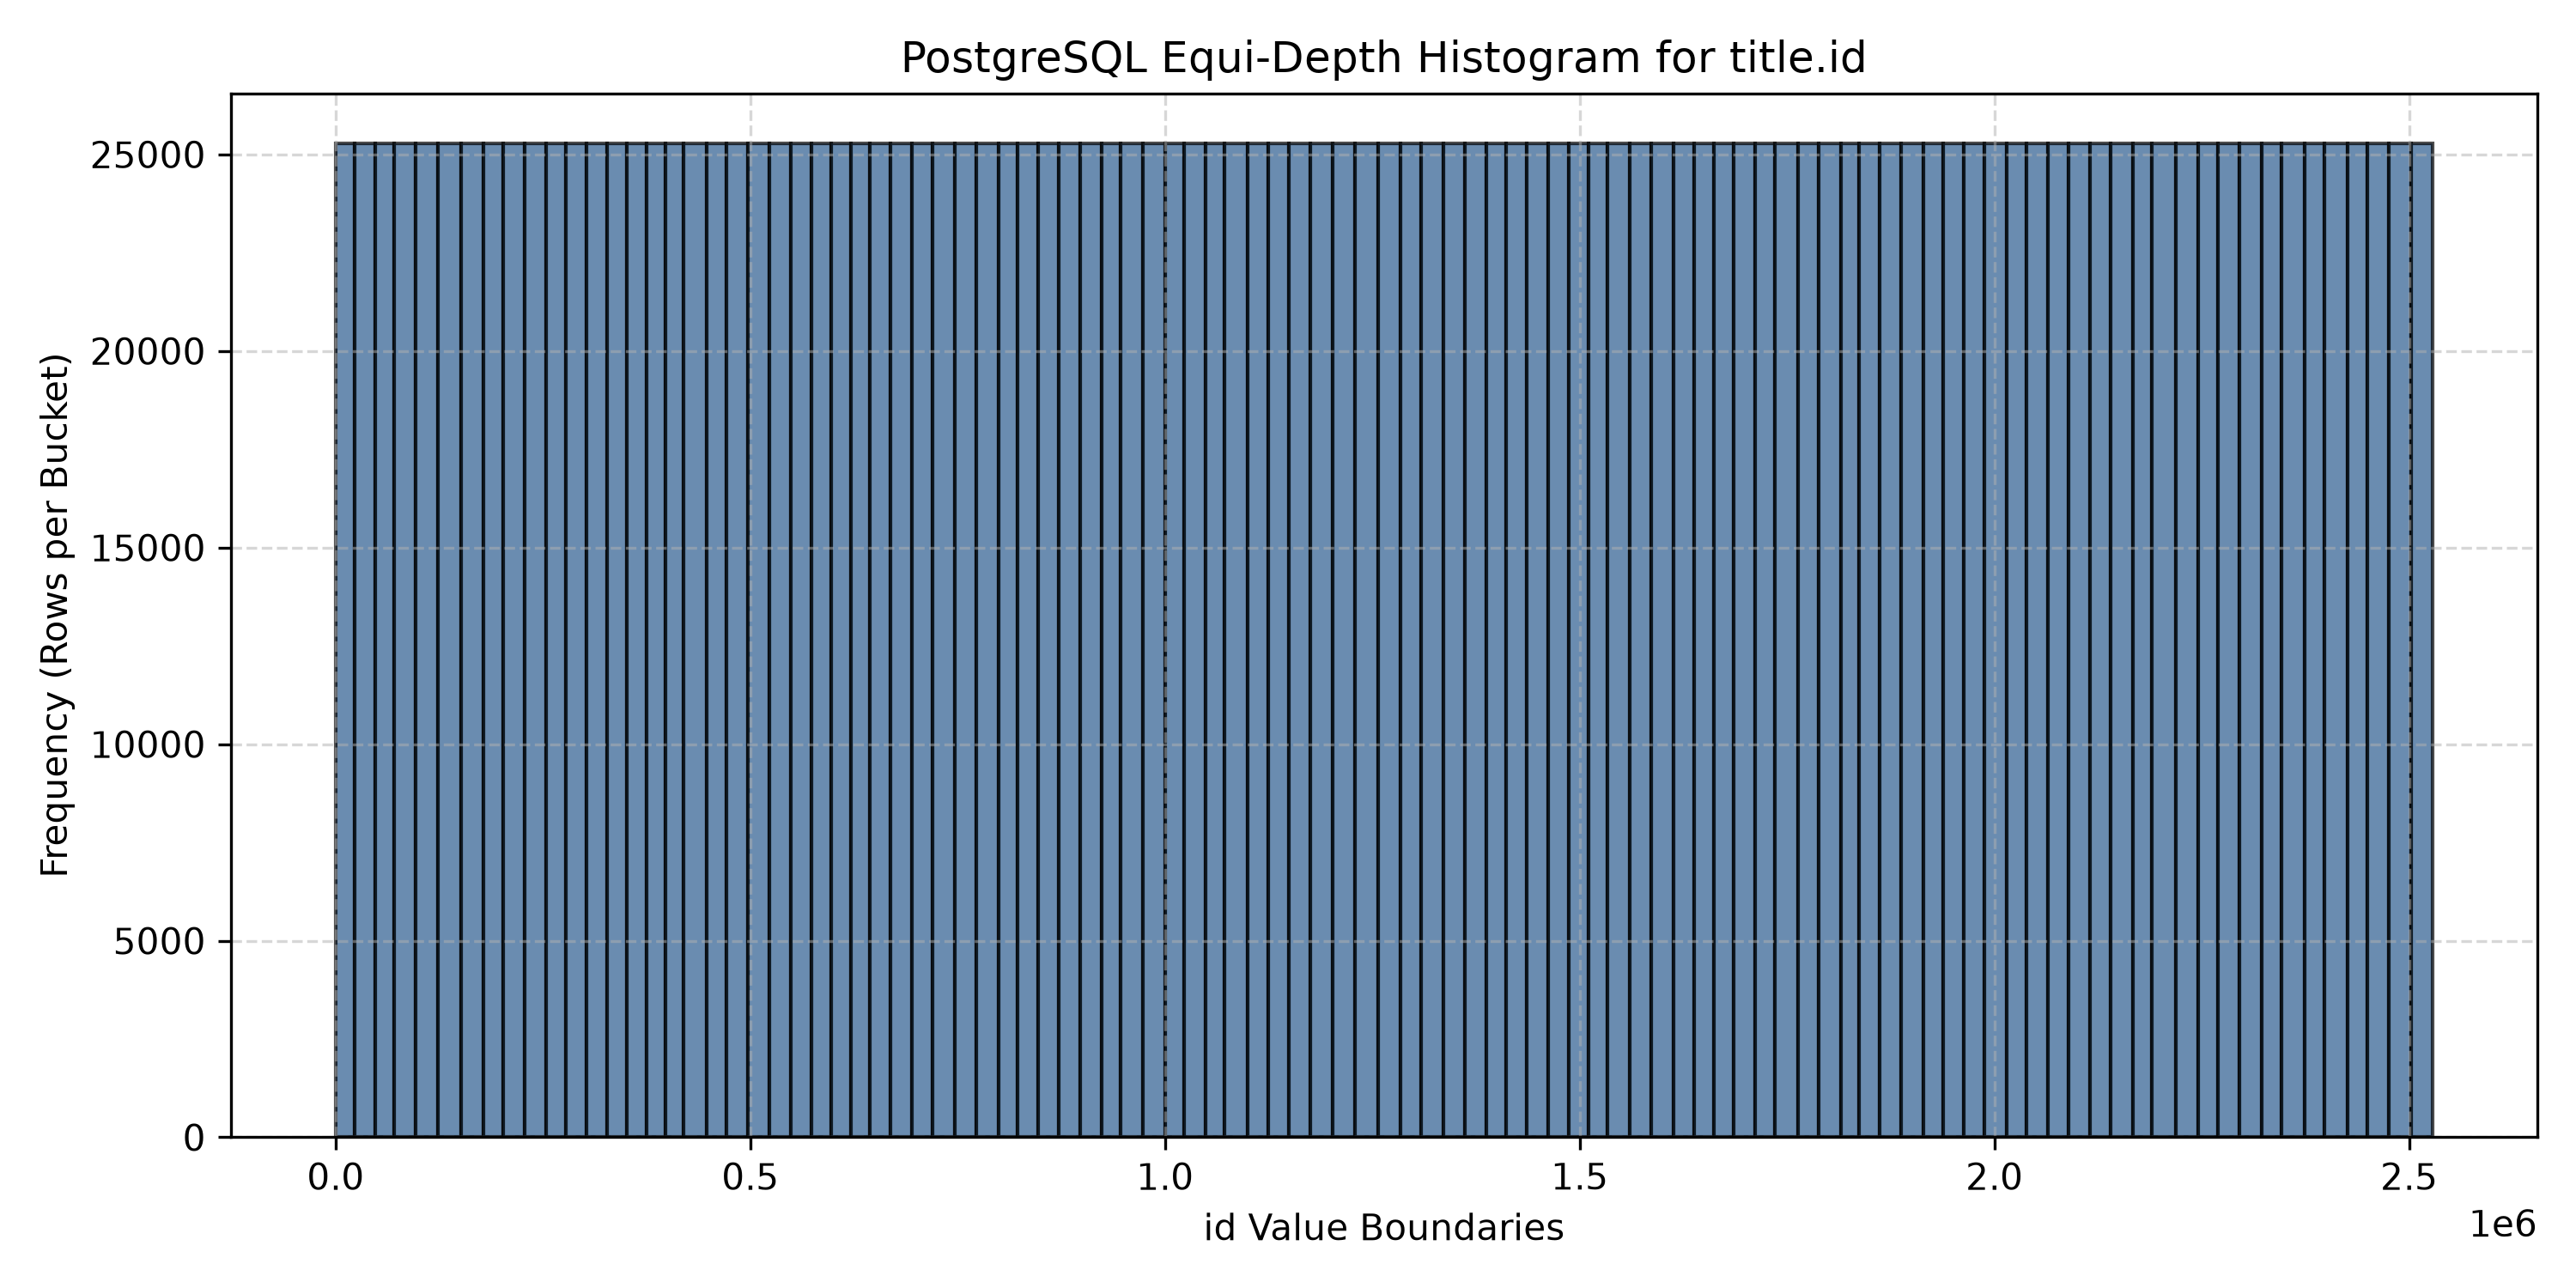
\includegraphics[width=0.85\textwidth]{q1_histogram_id.png}
\caption{Histogram for title.id}
\end{figure}

\begin{figure}[H]
\centering
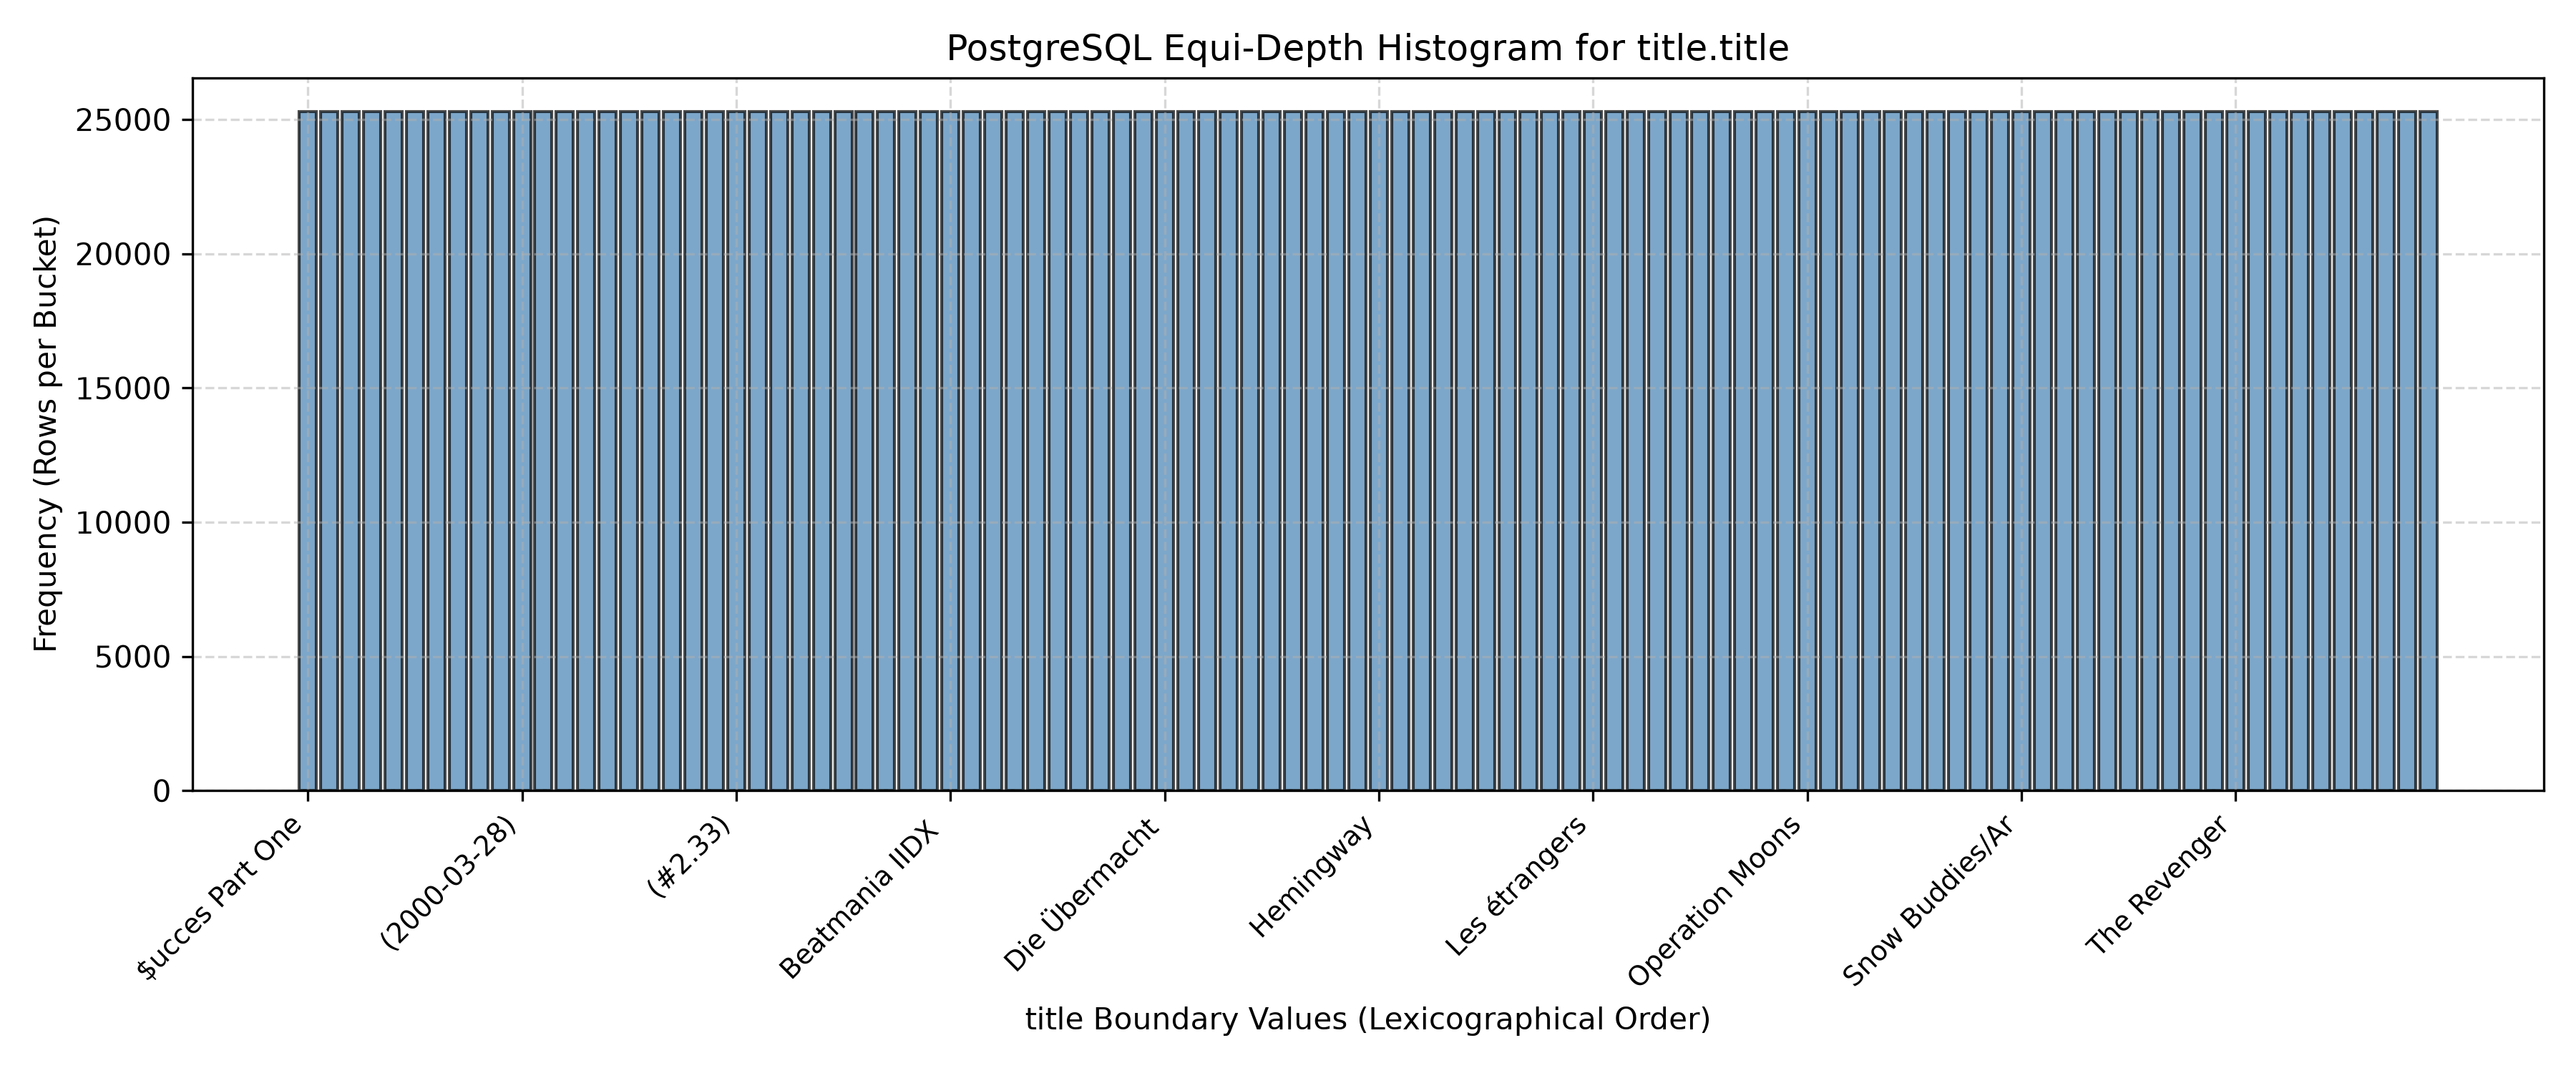
\includegraphics[width=0.85\textwidth]{q1_histogram_title.png}
\caption{Histogram for title.title}
\end{figure}

\subsubsection{7. Max Selectivity Error}
\begin{itemize}
\item \textbf{Max Selectivity Error}: Since \texttt{default\_statistics\_target} is 100, there are 100 buckets. Therefore, the maximum selectivity error for a range query is bounded by:
\end{itemize}
\[ \text{Max Error} \le \frac{1}{B} = \frac{1}{100} = 0.01 \quad (1.0\%) \]

For evaluated queries(q9), the observed maximum selectivity error is \textbf{0.8374\%} (0.008374), which strictly satisfies $\text{Max Error} \le 1.0\%$.


\hrule

\subsubsection{8: Selectivity Estimation for Text Columns}
Selectivity estimate is done for range query on text column such as “title” in PSQL such as:

*The engine scans the \texttt{histogram\_bounds} array stored under pg\_stats to locate the specific bucket where the target string  is, after that it counts all complete buckets preceding the target bucket. Each full bucket represents a fixed fraction of total rows (1/B). For the target bucket, PostgreSQL converts initial string bytes into floating-point numbers in $[0.0, 1.0]$ range for interpolation as explain in part 4,  assuming uniform distribution inside the target bucket, it calculates the target's position using:


\[ \text{Fraction} = \frac{\text{Query Value} - \text{Bucket Min}}{\text{Bucket Max} - \text{Bucket Min}} \]

\begin{itemize}
\item   Final Calculation is done by adding the fractional bucket estimate to the sum of preceding full buckets to get the final estimated selectivity.
\end{itemize}

\subsubsection{9: Estimated vs. Actual Selectivities}

To calculate estimated and actual selectivities of the queries and moreover there accuracy we compare estimated rows (from \texttt{EXPLAIN}) against actual rows (from \texttt{EXPLAIN ANALYZE}).

Total row count ($N$) for the \texttt{title} table is 2,528,312.


\textbf{Query 1: \texttt{title < 'Race'}}

\begin{lstlisting}[language=sql]
EXPLAIN ANALYZE SELECT * FROM title WHERE title.title < 'Race';
\end{lstlisting}

\begin{itemize}
\item \textbf{Actual Selectivity:} The query physically returned 1,918,141 matching rows: $S_{\text{act}} = \frac{1918141}{2528312} \approx 0.7587$ (75.87\%).
\end{itemize}

\begin{lstlisting}[language=sql]
EXPLAIN SELECT * FROM title WHERE title.title < 'Race';
\end{lstlisting}

\begin{itemize}
\item \textbf{Estimated Selectivity:} The planner estimated 1,939,313 rows: $S_{\text{est}} = \frac{1939313}{2528312} \approx 0.7670$ (76.70\%).
\end{itemize}

\begin{itemize}
\item \textbf{Observation:} The absolute error is roughly 0.84\%.
\end{itemize}

\textbf{Query 2: \texttt{id < 350000}}

\begin{lstlisting}[language=sql]
EXPLAIN ANALYZE SELECT * FROM title WHERE title.id < '350000';
\end{lstlisting}

\begin{itemize}
\item \textbf{Actual Selectivity:} The query returned 349,999 matching rows: $S_{\text{act}} = \frac{349999}{2528312} \approx 0.1384$ (13.84\%).
\end{itemize}

\begin{lstlisting}[language=sql]
EXPLAIN SELECT * FROM title WHERE title.id < '350000';
\end{lstlisting}

\begin{itemize}
\item \textbf{Estimated Selectivity:} The planner estimated 352,255 rows: $S_{\text{est}} = \frac{352255}{2528312} \approx 0.1393$ (13.93\%).
\end{itemize}

\begin{itemize}
\item \textbf{Observation:} The absolute error here is about 0.09\%.
\end{itemize}

\hrule


\subsection{Q2. Optimal Serial Histogram Construction ($B=10$ Buckets)}

\subsubsection{1. Histogram Visualizations for Exact $N = 3000$ Samples (Slide-9 Upright Vertical Block Plots)}
*As defined in lecture Slide 9, a Serial Histogram sorts domain values by their ordered frequencies ($f(v_{(1)}) \le f(v_{(2)}) \le \dots \le f(v_{(m)})$) and partitions the frequency space to minimize frequency variance $\sum n_i V_i$. The upright vertical block plots below feature Frequencies on the X-axis (ordered ascending) and Value Set / Stacked Domain Elements on the Y-axis:*


\begin{figure}[H]
\centering
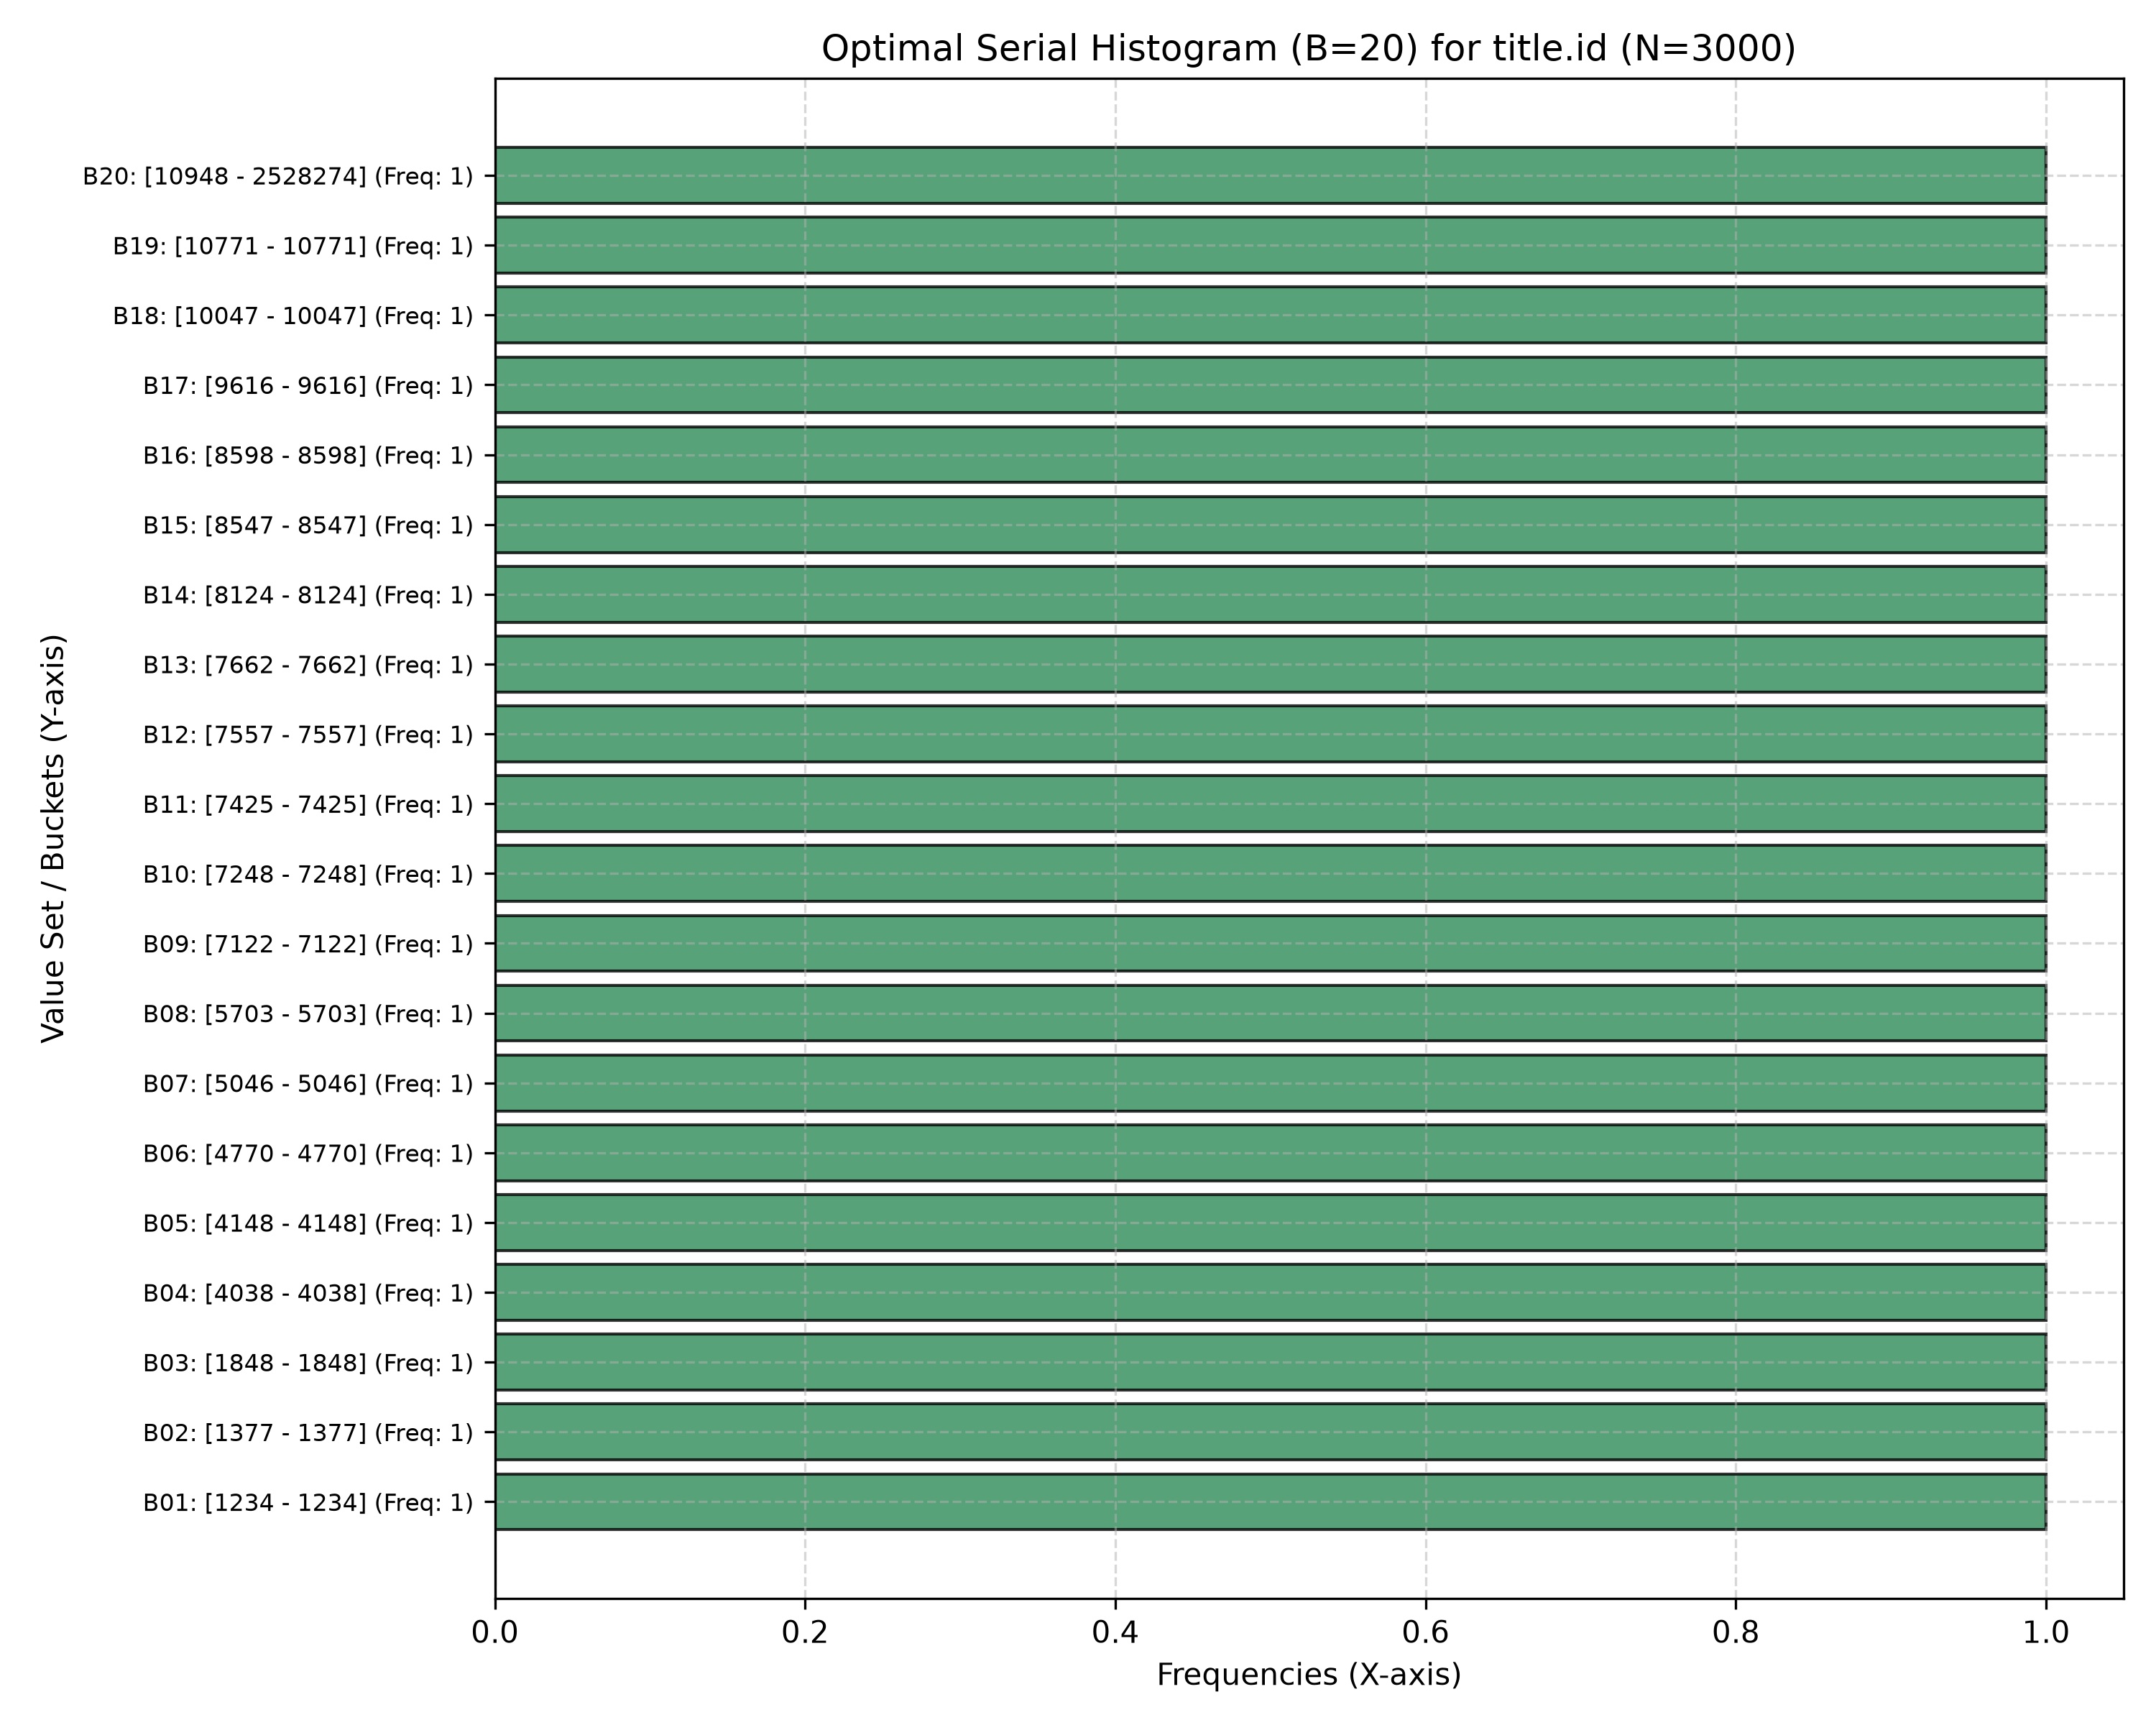
\includegraphics[width=0.85\textwidth]{q2_histogram_id_3000.png}
\caption{Correct Conceptual Plot for Unique title.id (N=3000)}
\end{figure}

\begin{figure}[H]
\centering
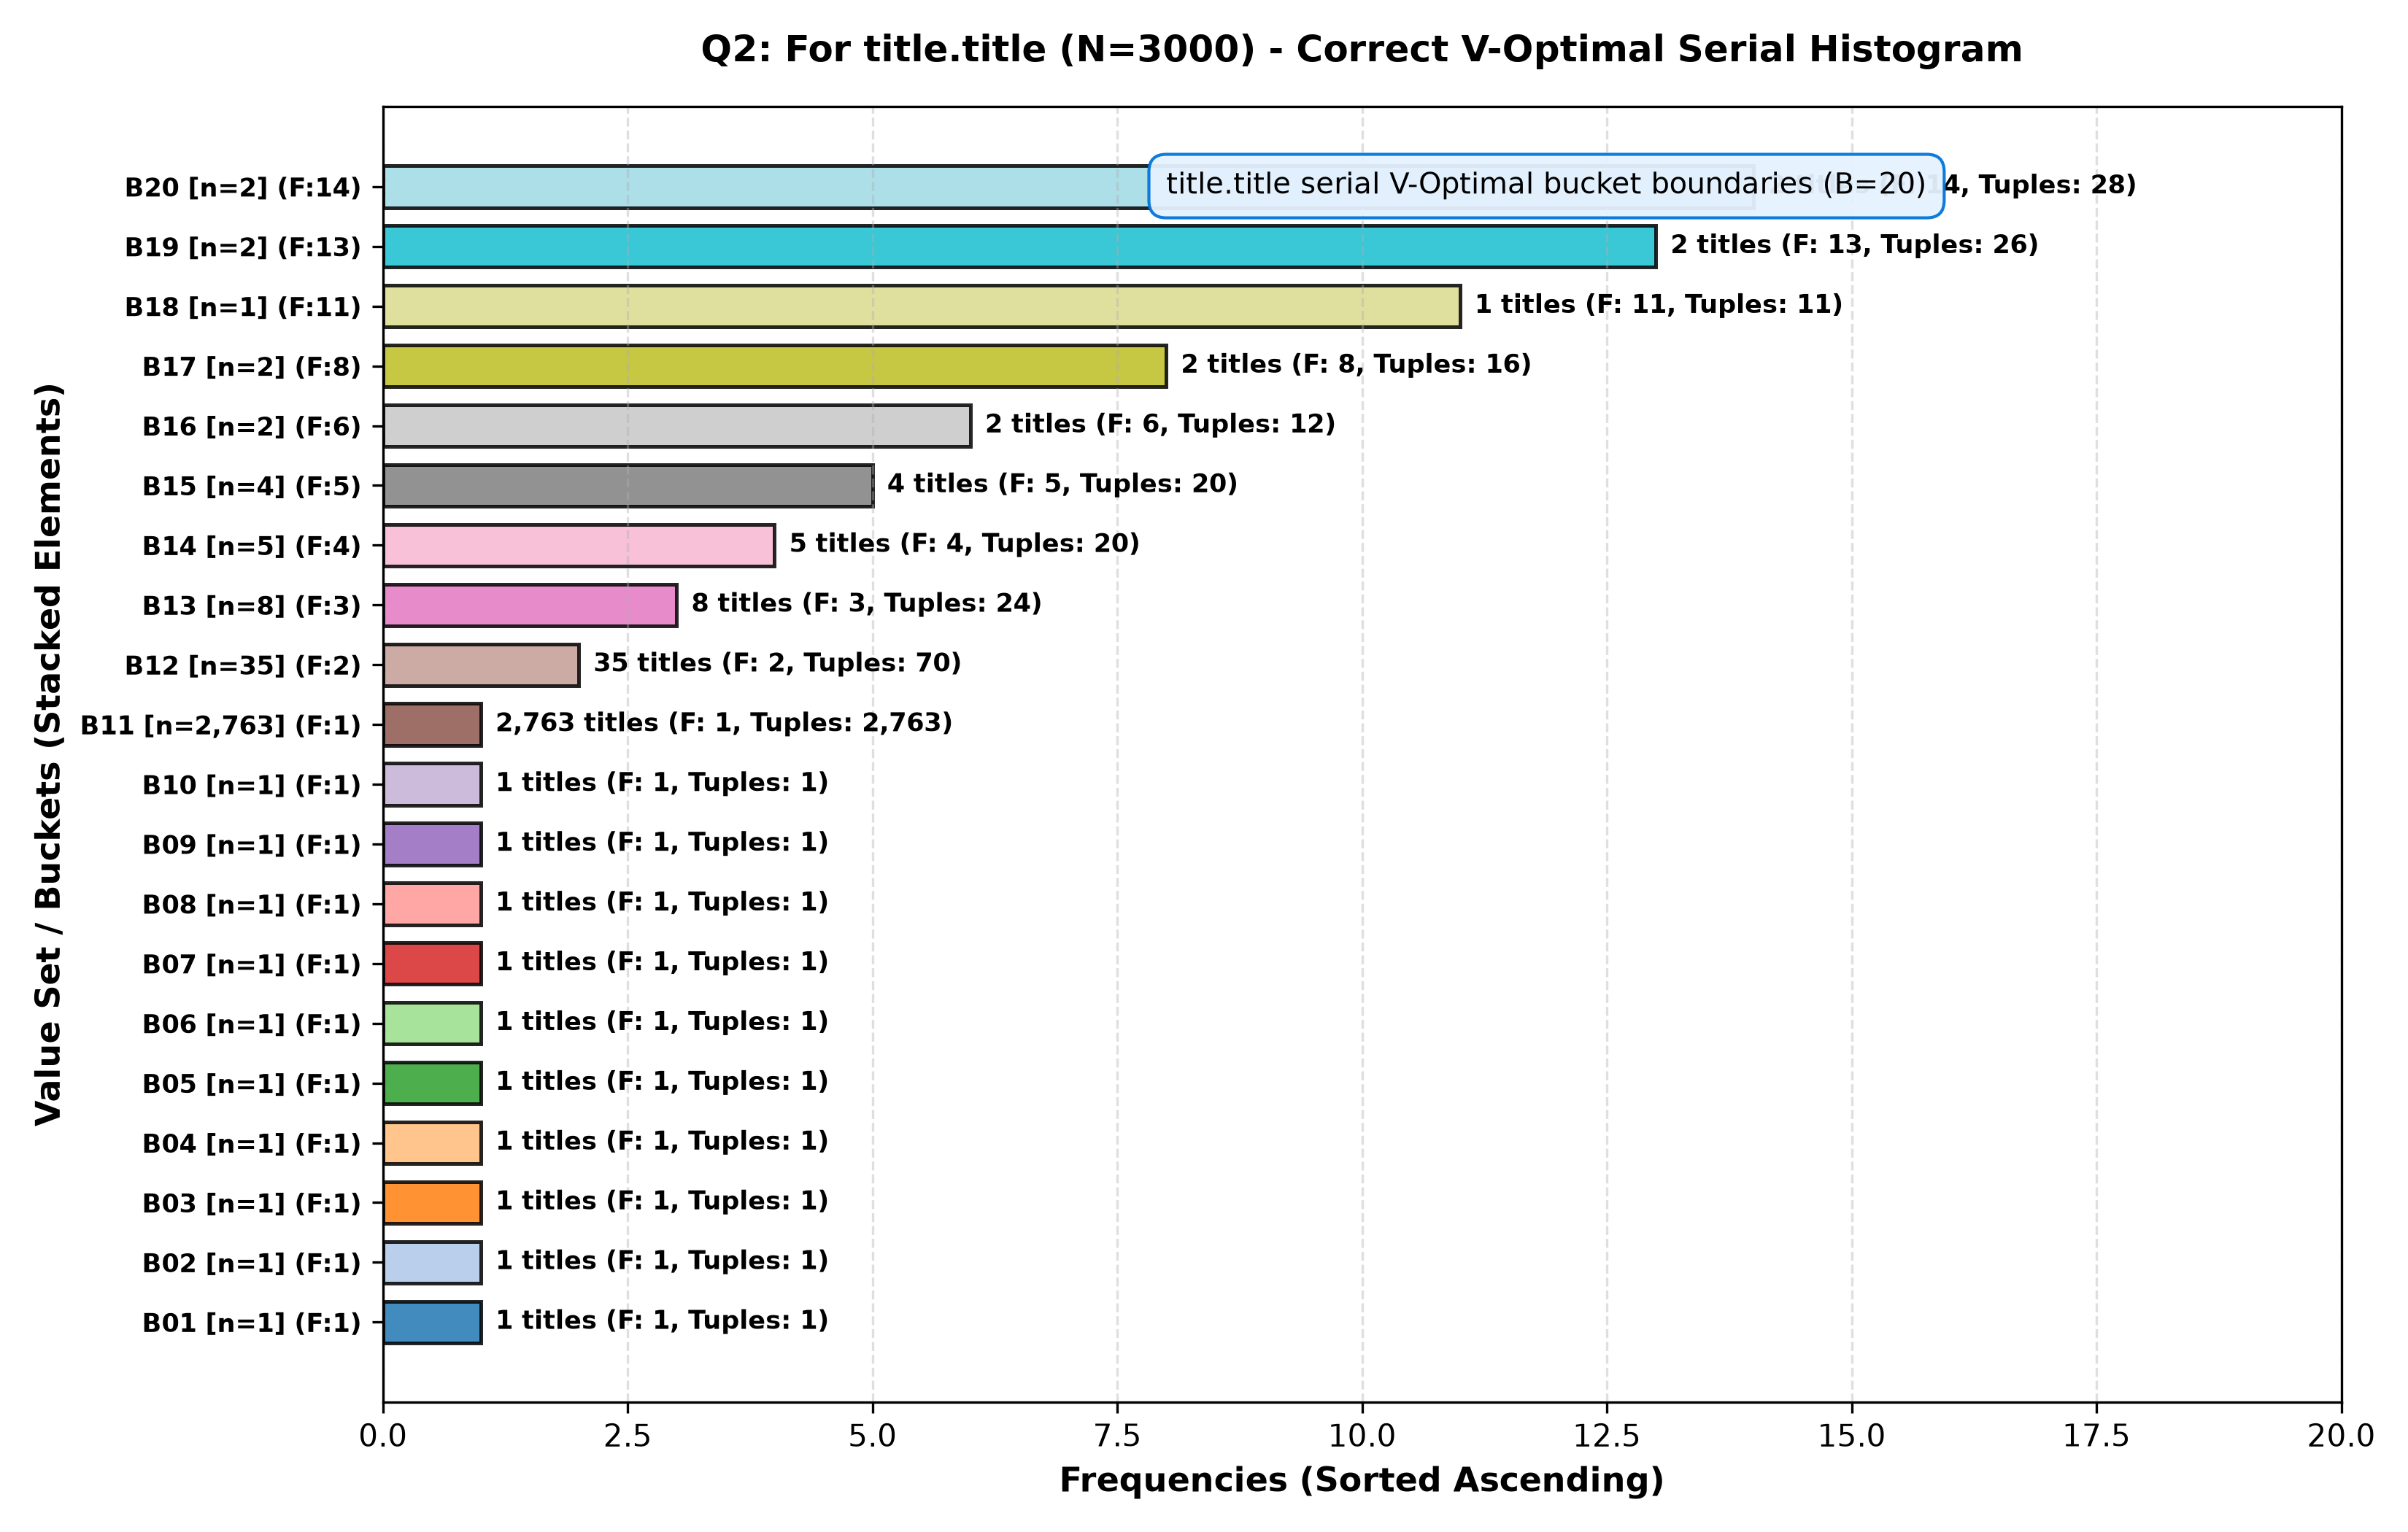
\includegraphics[width=0.85\textwidth]{q2_histogram_title_3000.png}
\caption{Q2: For title.title (N=3000) - Correct V-Optimal Serial Histogram}
\end{figure}

\subsubsection{2. Execution Build Time (Average over 3 Runs)}
\begin{itemize}
\item **Average Build Time for $N=3000$\textbf{: }0.2118 seconds\textbf{ (\texttt{id} column) / }0.3122 seconds** (\texttt{title} column)
\end{itemize}

\subsubsection{3. Frequency Bucket Boundaries ($N=3000$, $B=10$)}

The optimal serial histogram algorithm partitions the exact 3,000 samples into dynamic frequency buckets ($B=10$). The exact bucket value ranges, distinct domain value counts ($n_i$), and frequency distributions for both columns are listed below:


\paragraph{A. Column \texttt{id} Serial Frequency Bucket Boundaries ($N=3000$, $B=10$)}
{\begingroup
\small
\setlength{\tabcolsep}{4pt}
\begin{xltabular}{\textwidth}{C | C | C | C | C}
\toprule
\textbf{Bucket \#} & \textbf{Value Range (\texttt{id})} & \textbf{Distinct Values ($n_i$)} & \textbf{Frequency Range} & \textbf{Average Frequency ($ar{f}_i$)} \\
\midrule
\endfirsthead
\toprule
\textbf{Bucket \#} & \textbf{Value Range (\texttt{id})} & \textbf{Distinct Values ($n_i$)} & \textbf{Frequency Range} & \textbf{Average Frequency ($ar{f}_i$)} \\
\midrule
\endfirsthead
\endhead
\bottomrule
\endfoot
\bottomrule
\endlastfoot
Bucket 01 & [\texttt{1,234} - \texttt{2,528,274}] & 3000 & 1 & 1.00 \\
\end{xltabular}
\endgroup}


\paragraph{B. Column \texttt{title} Serial Frequency Bucket Boundaries ($N=3000$, $B=10$)}
{\begingroup
\small
\setlength{\tabcolsep}{4pt}
\begin{xltabular}{\textwidth}{C | C | C | C | C}
\toprule
\textbf{Bucket \#} & \textbf{Value Range (\texttt{title})} & \textbf{Distinct Values ($n_i$)} & \textbf{Frequency Range} & \textbf{Average Frequency ($ar{f}_i$)} \\
\midrule
\endfirsthead
\toprule
\textbf{Bucket \#} & \textbf{Value Range (\texttt{title})} & \textbf{Distinct Values ($n_i$)} & \textbf{Frequency Range} & \textbf{Average Frequency ($ar{f}_i$)} \\
\midrule
\endfirsthead
\endhead
\bottomrule
\endfoot
\bottomrule
\endlastfoot
Bucket 01 & [\texttt{"\textbackslash{}\$\#!+ Happens"} ... \texttt{"Ônna no kaôyaku"}] & 2773 & 1 & 1.00 \\
Bucket 02 & [\texttt{"(\#1.132)"} ... \texttt{"The Box"}] & 35 & 2 & 2.00 \\
Bucket 03 & [\texttt{"(\#1.118)"} ... \texttt{"(\#4.1)"}] & 8 & 3 & 3.00 \\
Bucket 04 & [\texttt{"(\#1.11)"} ... \texttt{"(\#3.1)"}] & 5 & 4 & 4.00 \\
Bucket 05 & [\texttt{"(\#1.10)"} ... \texttt{"Pilot"}] & 4 & 5 & 5.00 \\
Bucket 06 & [\texttt{"(\#1.7)"} ... \texttt{"(\#1.9)"}] & 2 & 6 & 6.00 \\
Bucket 07 & [\texttt{"(\#1.6)"} ... \texttt{"(\#1.8)"}] & 2 & 8 & 8.00 \\
Bucket 08 & [\texttt{"(\#1.5)"} ... \texttt{"(\#1.5)"}] & 1 & 11 & 11.00 \\
Bucket 09 & [\texttt{"(\#1.1)"} ... \texttt{"(\#1.2)"}] & 2 & 13 & 13.00 \\
Bucket 10 & [\texttt{"(\#1.3)"} ... \texttt{"(\#1.4)"}] & 2 & 14 & 14.00 \\
\end{xltabular}
\endgroup}


\subsubsection{4. 3-Run Selectivity Error Calculation \& Average ($N=3000$)}

As required to account for sample randomness, the selectivity error evaluation was executed across \textbf{3 independent runs} (with exact sample size $N=3000$). All three run errors are listed below along with their computed average:


\paragraph{A. 3-Run Max Selectivity Error Summary ($N=3000$)}
{\begingroup
\small
\setlength{\tabcolsep}{4pt}
\begin{xltabular}{\textwidth}{C | C | C | C | C}
\toprule
\textbf{Column} & \textbf{Run 1 Max Error} & \textbf{Run 2 Max Error} & \textbf{Run 3 Max Error} & \textbf{\textbf{Average Max Selectivity Error}} \\
\midrule
\endfirsthead
\toprule
\textbf{Column} & \textbf{Run 1 Max Error} & \textbf{Run 2 Max Error} & \textbf{Run 3 Max Error} & \textbf{\textbf{Average Max Selectivity Error}} \\
\midrule
\endfirsthead
\endhead
\bottomrule
\endfoot
\bottomrule
\endlastfoot
\texttt{id} & \texttt{0.022444} & \texttt{0.009556} & \texttt{0.009889} & \textbf{\texttt{0.013963}} (1.3963\%) \\
\texttt{title} & \texttt{0.612556} & \texttt{0.609000} & \texttt{0.616667} & \textbf{\texttt{0.612741}} (61.2741\%) \\
\end{xltabular}
\endgroup}


\paragraph{B. Quantile-by-Quantile Error Evaluation Table for Run 1 ($N=3000, B=10$)}
{\begingroup
\footnotesize
\setlength{\tabcolsep}{3.5pt}
\begin{xltabular}{\textwidth}{C | C | C | C | C | C | C}
\toprule
\textbf{Index ($k$)} & \textbf{Query Threshold ($q_k$)} & \textbf{Actual Count ($A$)} & \textbf{Actual Selectivity ($S_{\text{act}}$)} & \textbf{Estimated Count ($E$)} & \textbf{Estimated Selectivity ($S_{\text{est}}$)} & \textbf{Absolute Error $\vert S_{\text{est}} - S_{\text{act}} \vert$} \\
\midrule
\endfirsthead
\toprule
\textbf{Index ($k$)} & \textbf{Query Threshold ($q_k$)} & \textbf{Actual Count ($A$)} & \textbf{Actual Selectivity ($S_{\text{act}}$)} & \textbf{Estimated Count ($E$)} & \textbf{Estimated Selectivity ($S_{\text{est}}$)} & \textbf{Absolute Error $\vert S_{\text{est}} - S_{\text{act}} \vert$} \\
\midrule
\endfirsthead
\endhead
\bottomrule
\endfoot
\bottomrule
\endlastfoot
$q_{0}$ & \texttt{1,234.0} & 1 & 0.000333 & 0.00 & 0.000000 & 0.000333 \\
$q_{1}$ & \texttt{282,016.2} & 352 & 0.117333 & 333.33 & 0.111111 & 0.006222 \\
$q_{2}$ & \texttt{562,798.4} & 673 & 0.224333 & 666.67 & 0.222222 & 0.002111 \\
$q_{3}$ & \texttt{843,580.7} & 966 & 0.322000 & 1000.00 & 0.333333 & 0.011333 \\
$q_{4}$ & \texttt{1,124,362.9} & 1307 & 0.435667 & 1333.33 & 0.444444 & 0.008778 \\
$q_{5}$ & \texttt{1,405,145.1} & 1613 & 0.537667 & 1666.67 & 0.555556 & 0.017889 \\
$q_{6}$ & \texttt{1,685,927.3} & 1946 & 0.648667 & 2000.00 & 0.666667 & 0.018000 \\
$q_{7}$ & \texttt{1,966,709.6} & 2266 & 0.755333 & 2333.33 & 0.777778 & \textbf{0.022444} \\
$q_{8}$ & \texttt{2,247,491.8} & 2623 & 0.874333 & 2666.67 & 0.888889 & 0.014556 \\
$q_{9}$ & \texttt{2,528,274.0} & 3000 & 1.000000 & 3000.00 & 1.000000 & 0.000000 \\
\end{xltabular}
\endgroup}


\subsubsection{5. Histograms Across Exact Sample Sizes ($N = 1000, 3000, 5000$)}

Below are the optimal serial histogram visualizations ($B=10$) for exact sample sizes $N=1000$, $N=3000$, and $N=5000$:N=5000\$:


\paragraph{A. Sample Size $N = 1000$ Histograms}
\begin{figure}[H]
\centering
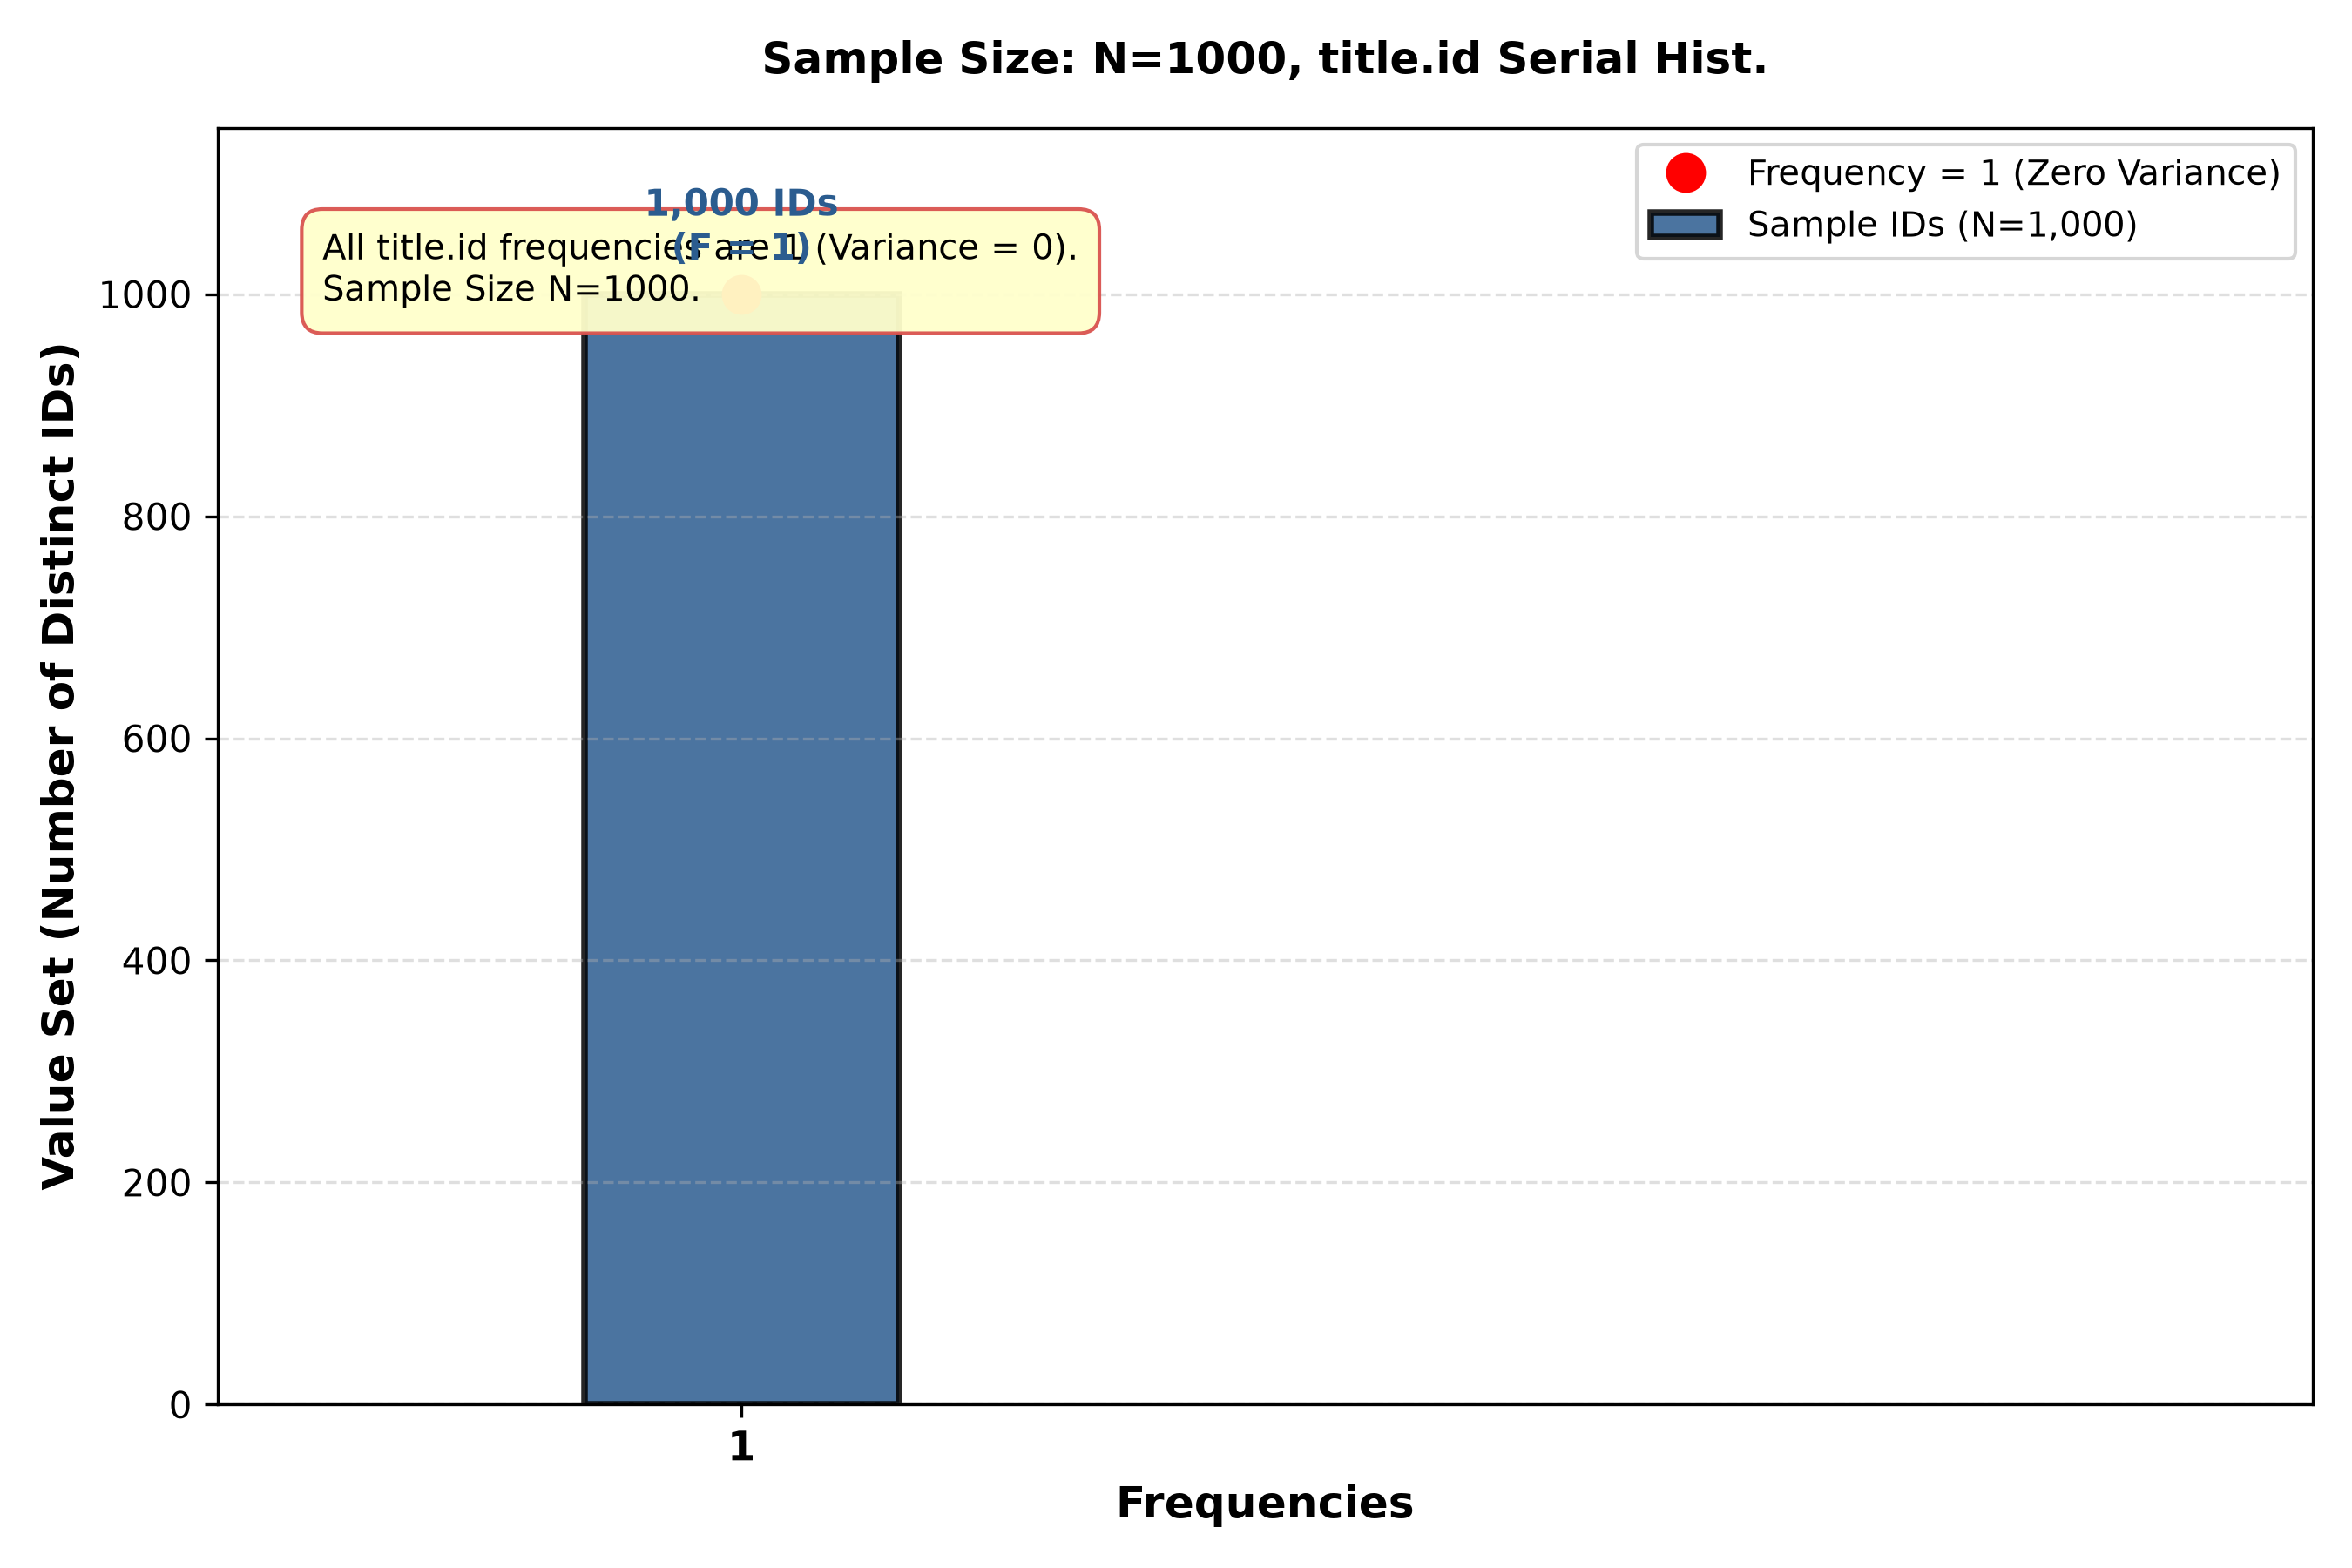
\includegraphics[width=0.85\textwidth]{q2_histogram_id_1000.png}
\caption{Sample Size: N=1000, title.id Serial Hist.}
\end{figure}

\begin{figure}[H]
\centering
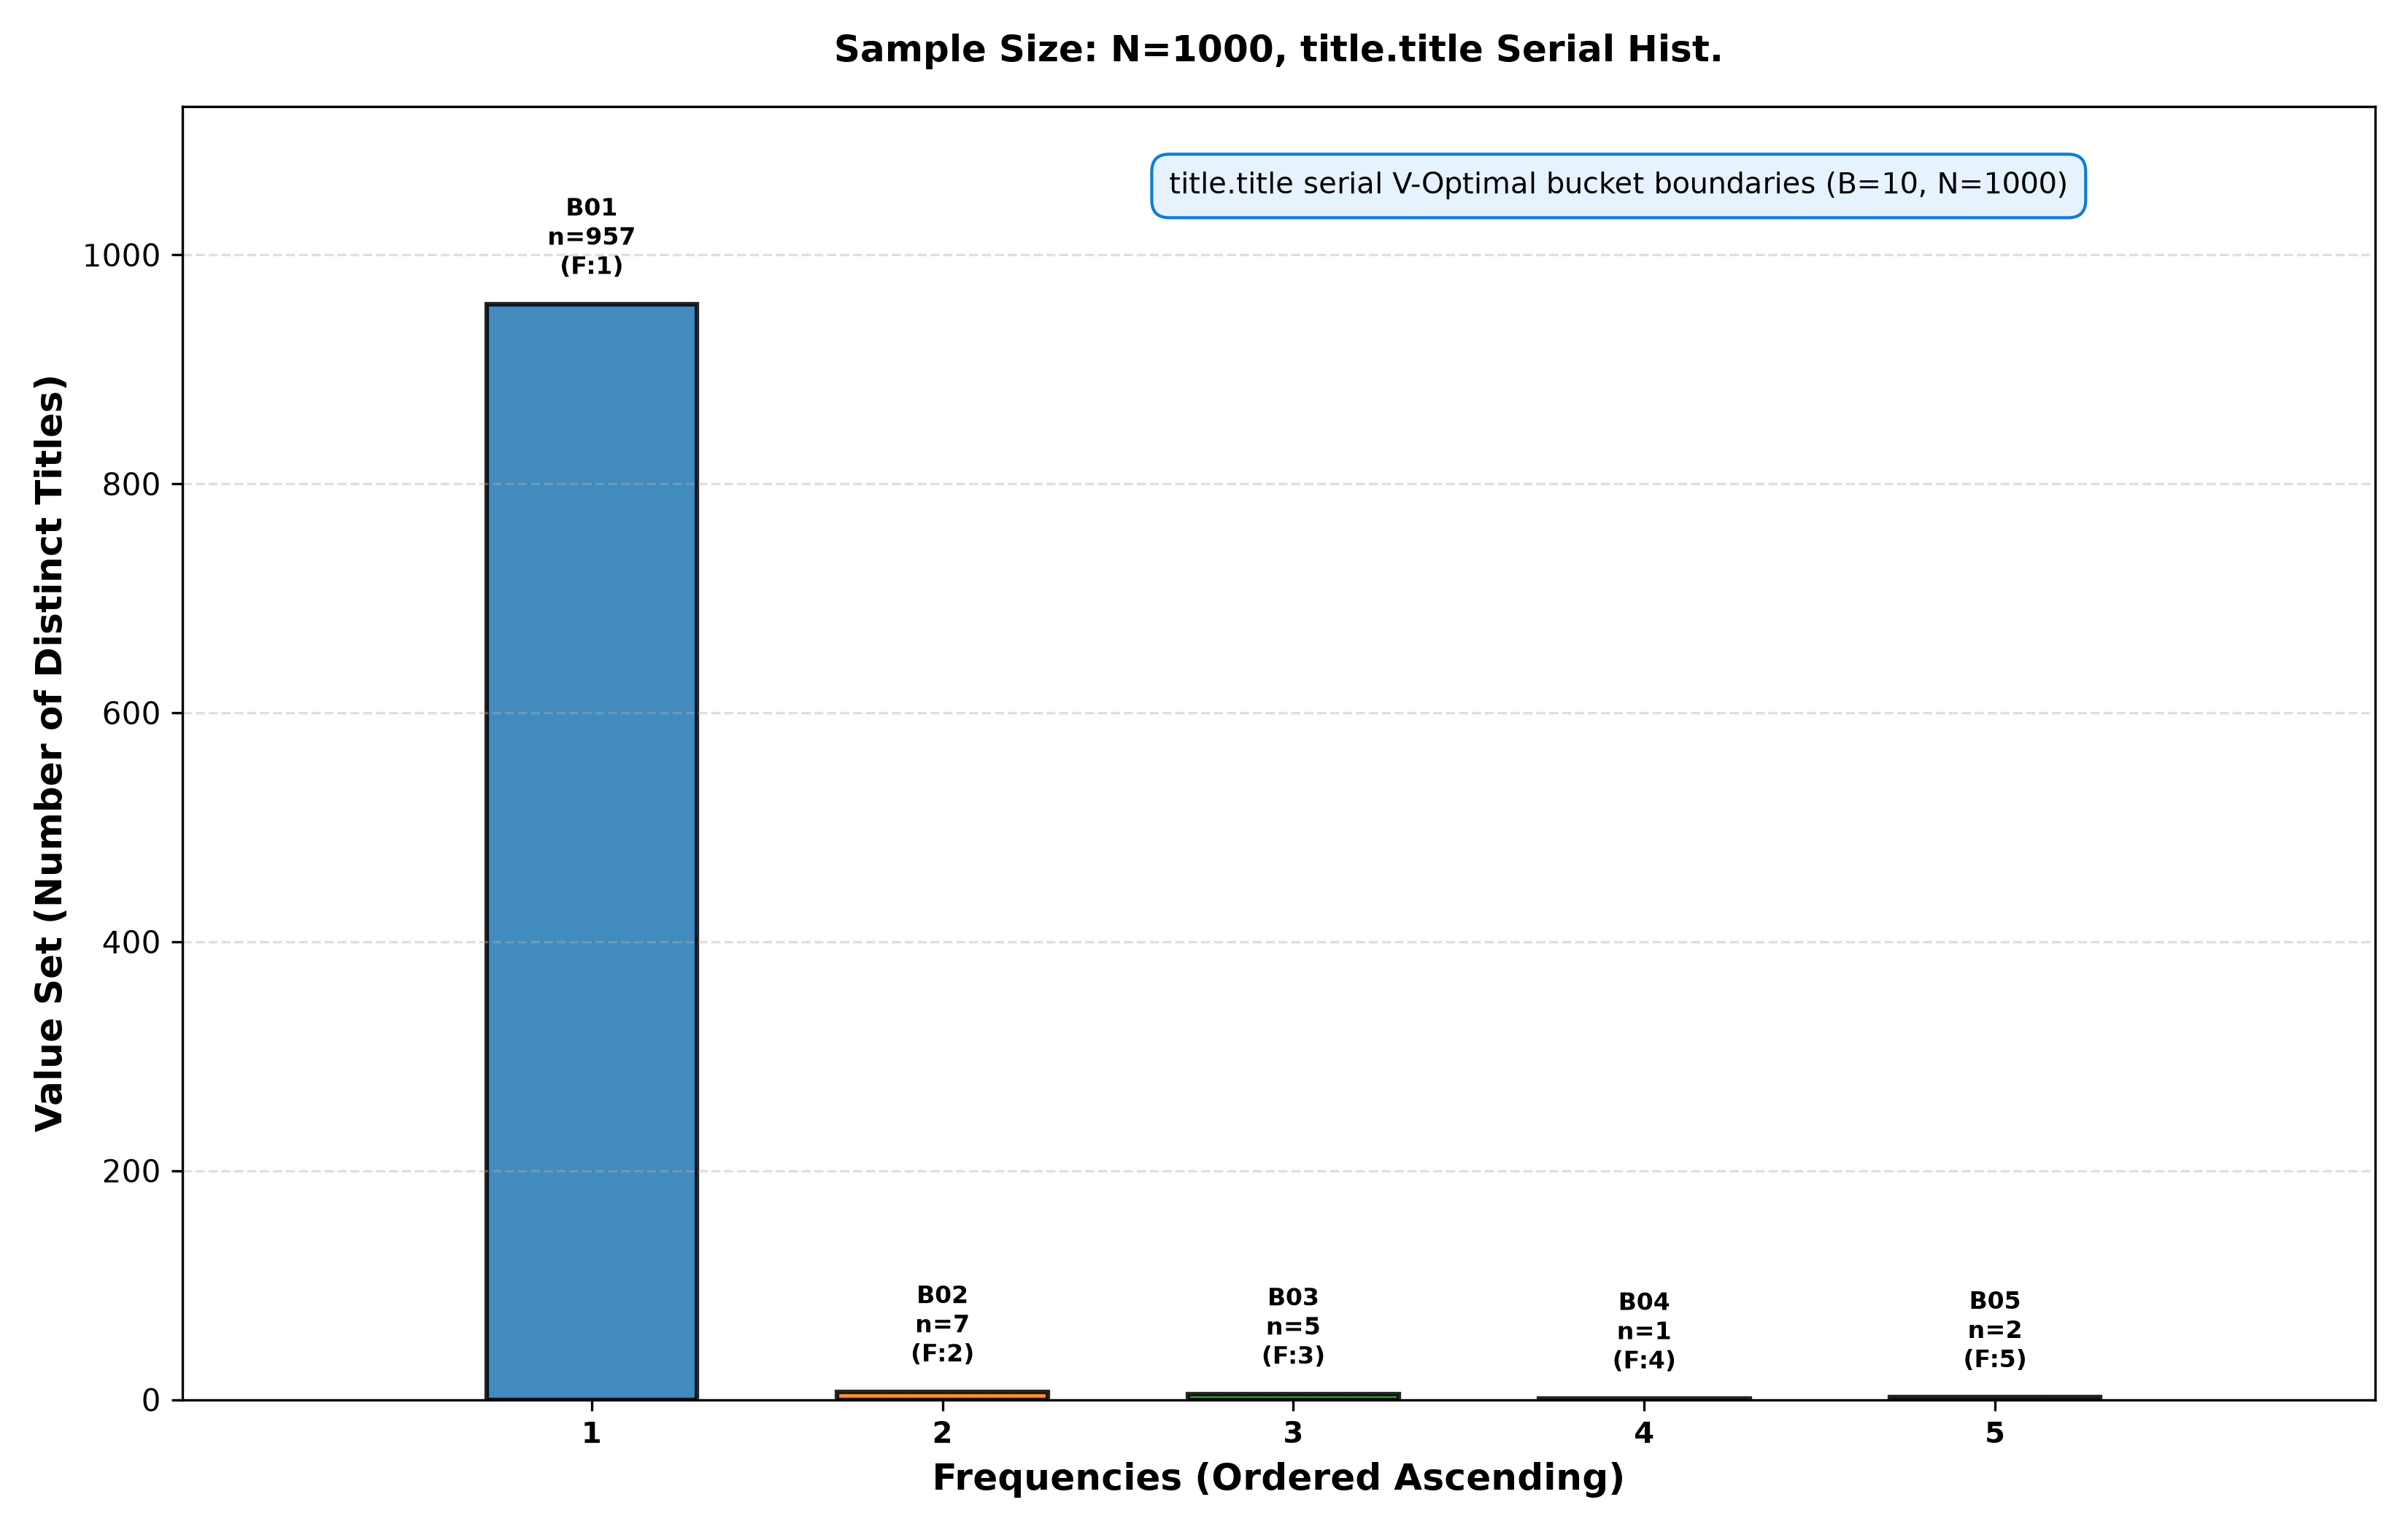
\includegraphics[width=0.85\textwidth]{q2_histogram_title_1000.png}
\caption{Sample Size: N=1000, title.title Serial Hist.}
\end{figure}

\paragraph{B. Sample Size $N = 3000$ Histograms}
\begin{figure}[H]
\centering
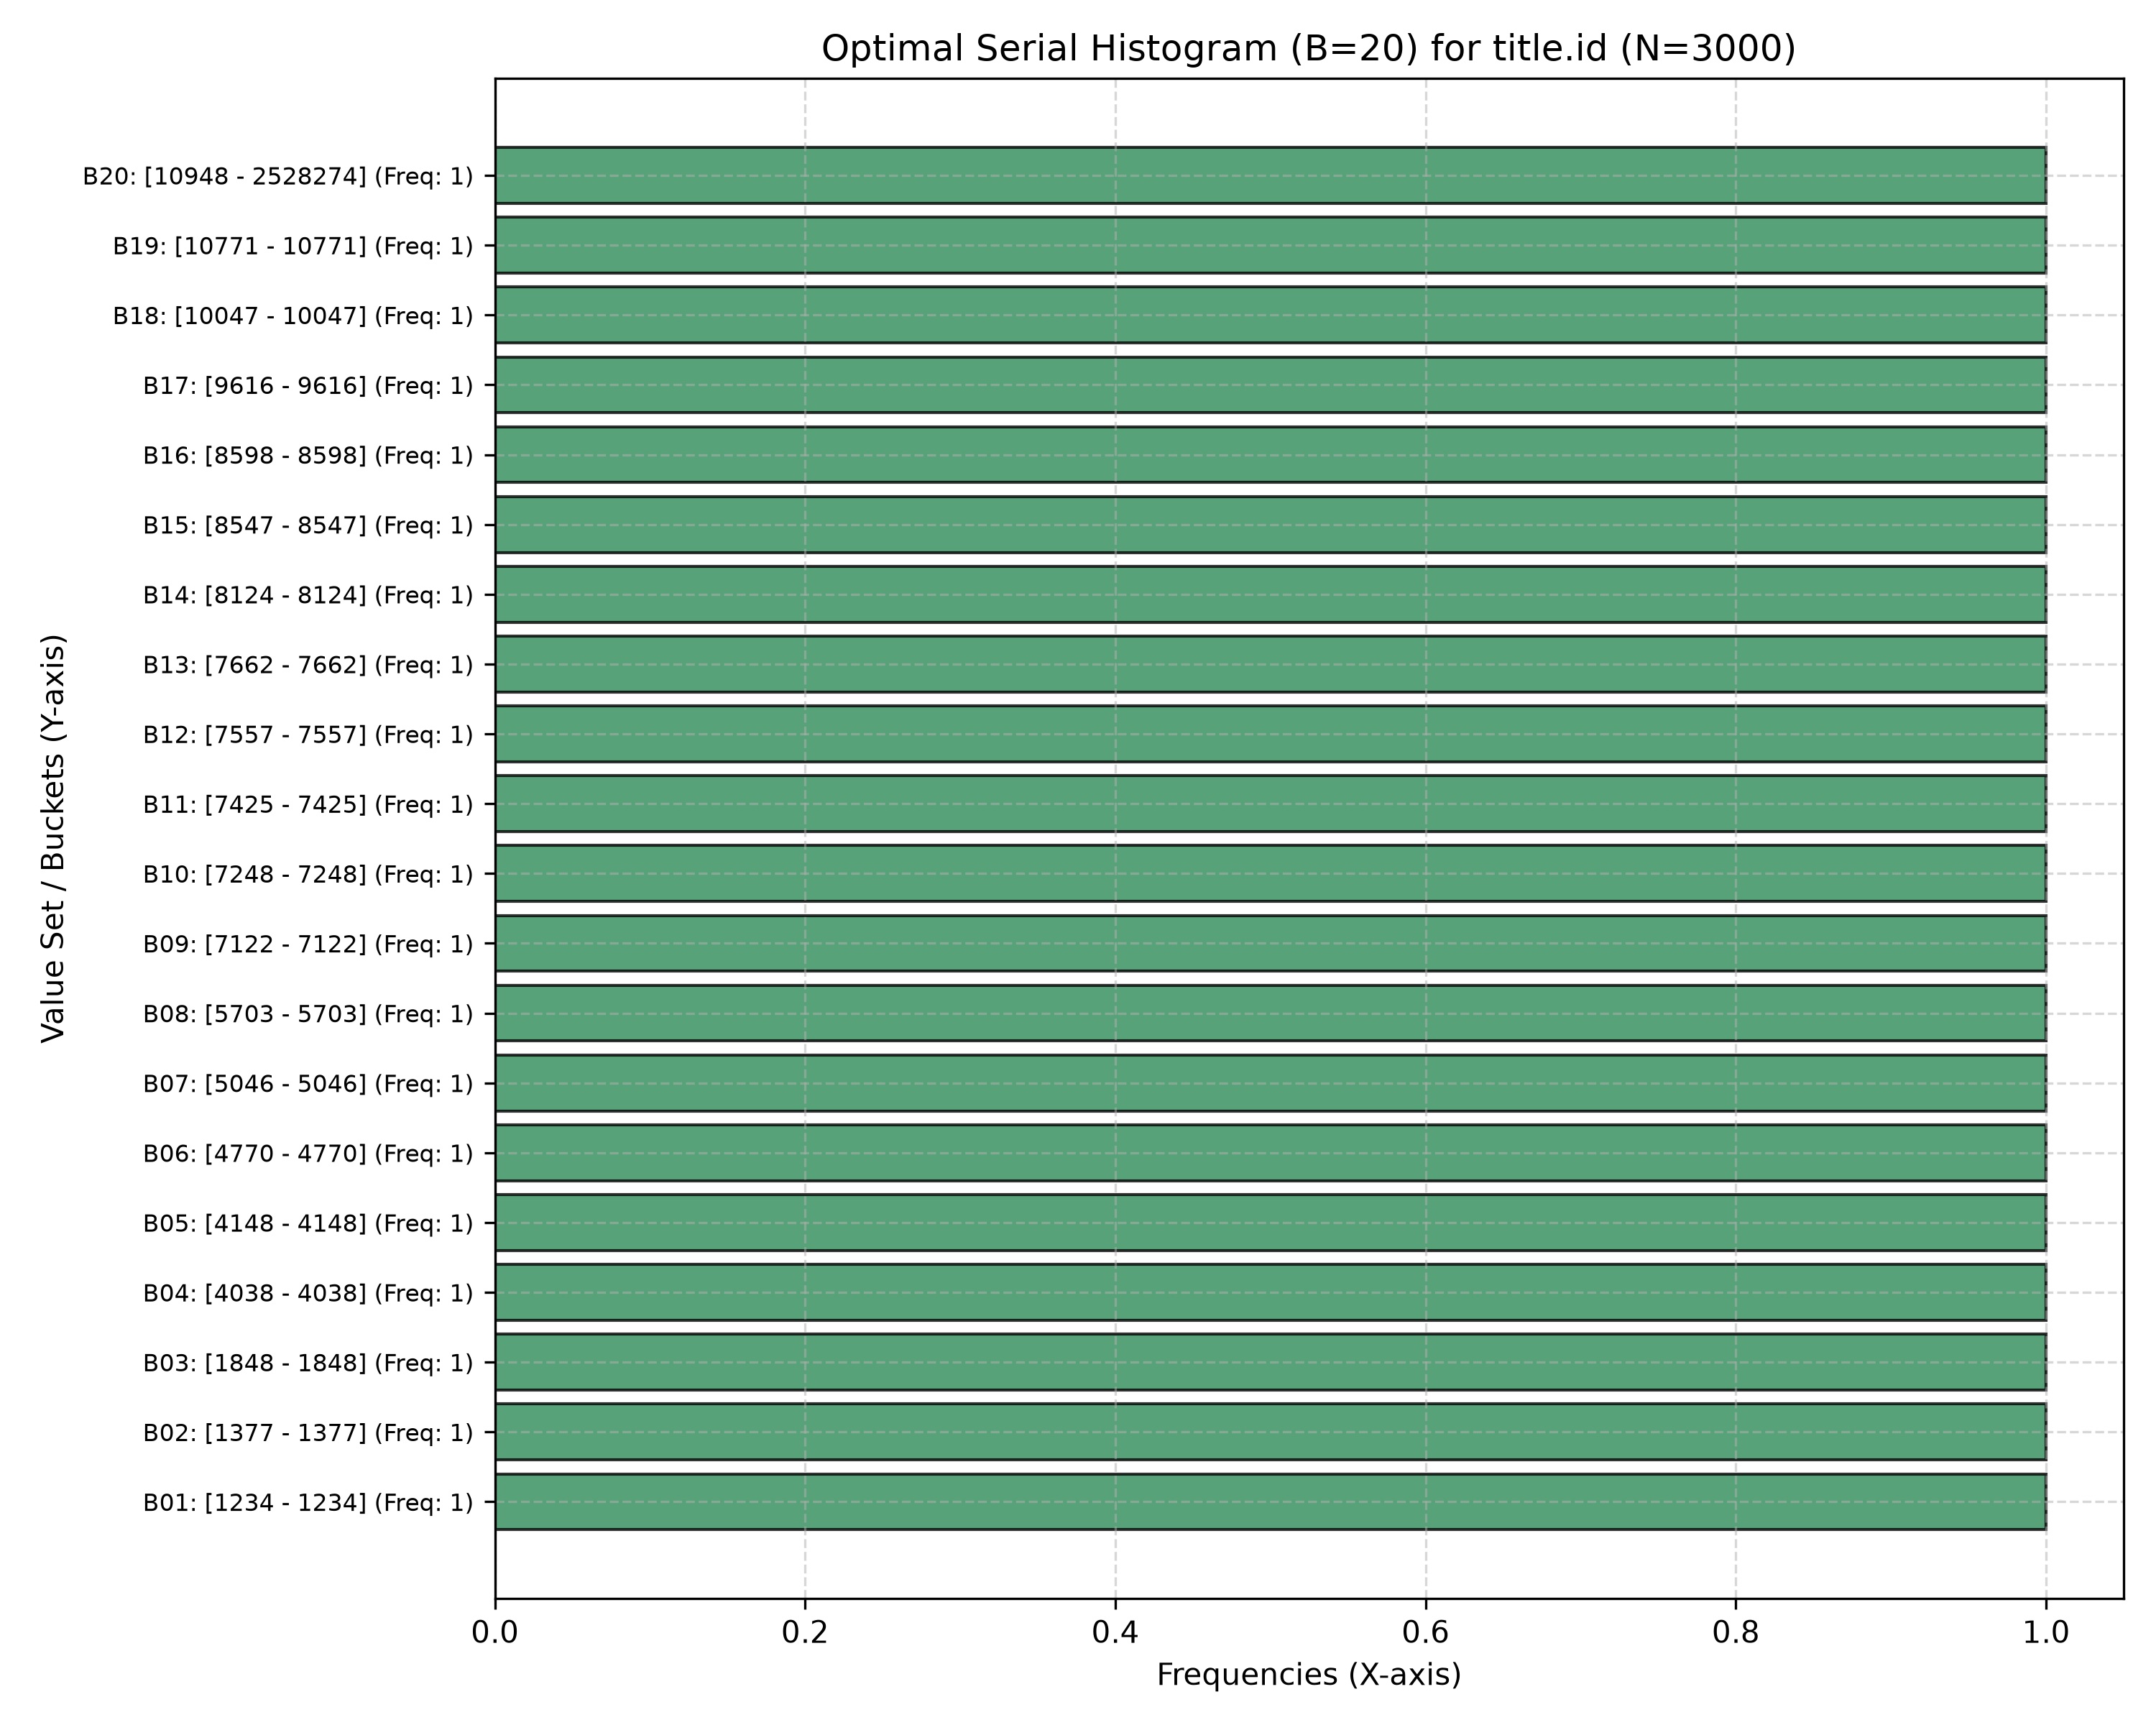
\includegraphics[width=0.85\textwidth]{q2_histogram_id_3000.png}
\caption{Correct Conceptual Plot for Unique title.id (N=3000)}
\end{figure}

\begin{figure}[H]
\centering
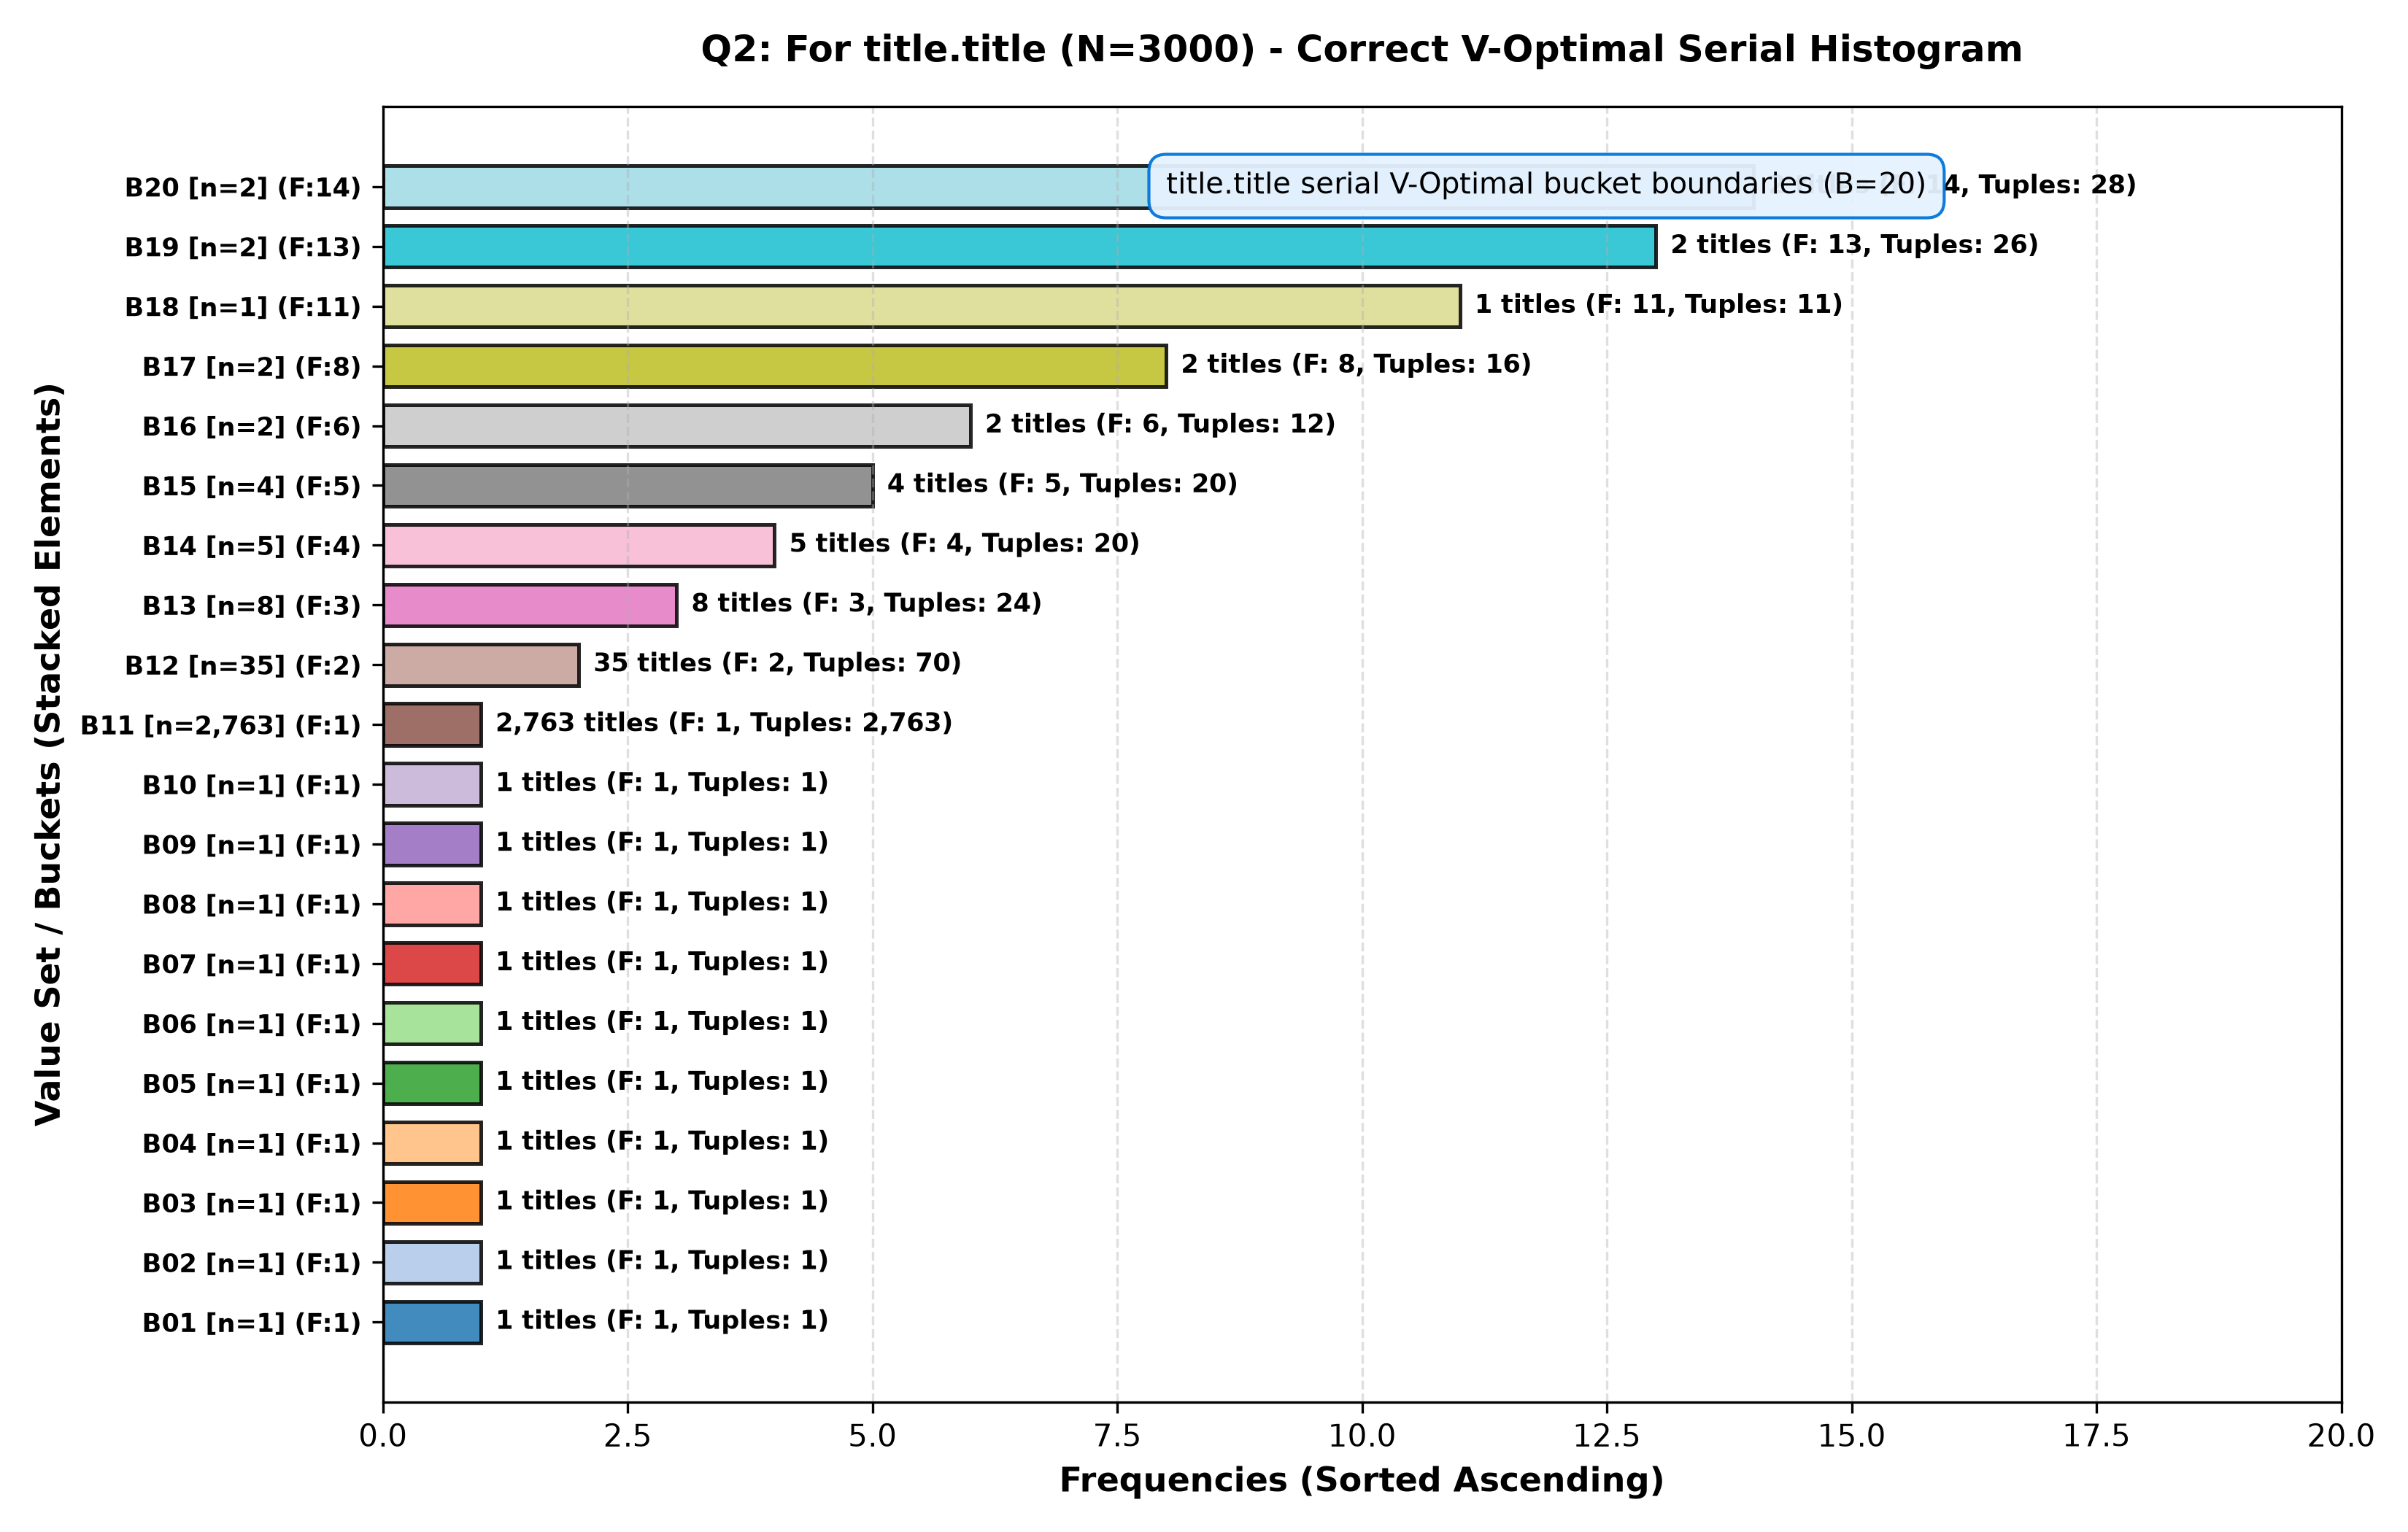
\includegraphics[width=0.85\textwidth]{q2_histogram_title_3000.png}
\caption{Q2: For title.title (N=3000) - Correct V-Optimal Serial Histogram}
\end{figure}

\paragraph{C. Sample Size $N = 5000$ Histograms}
\begin{figure}[H]
\centering
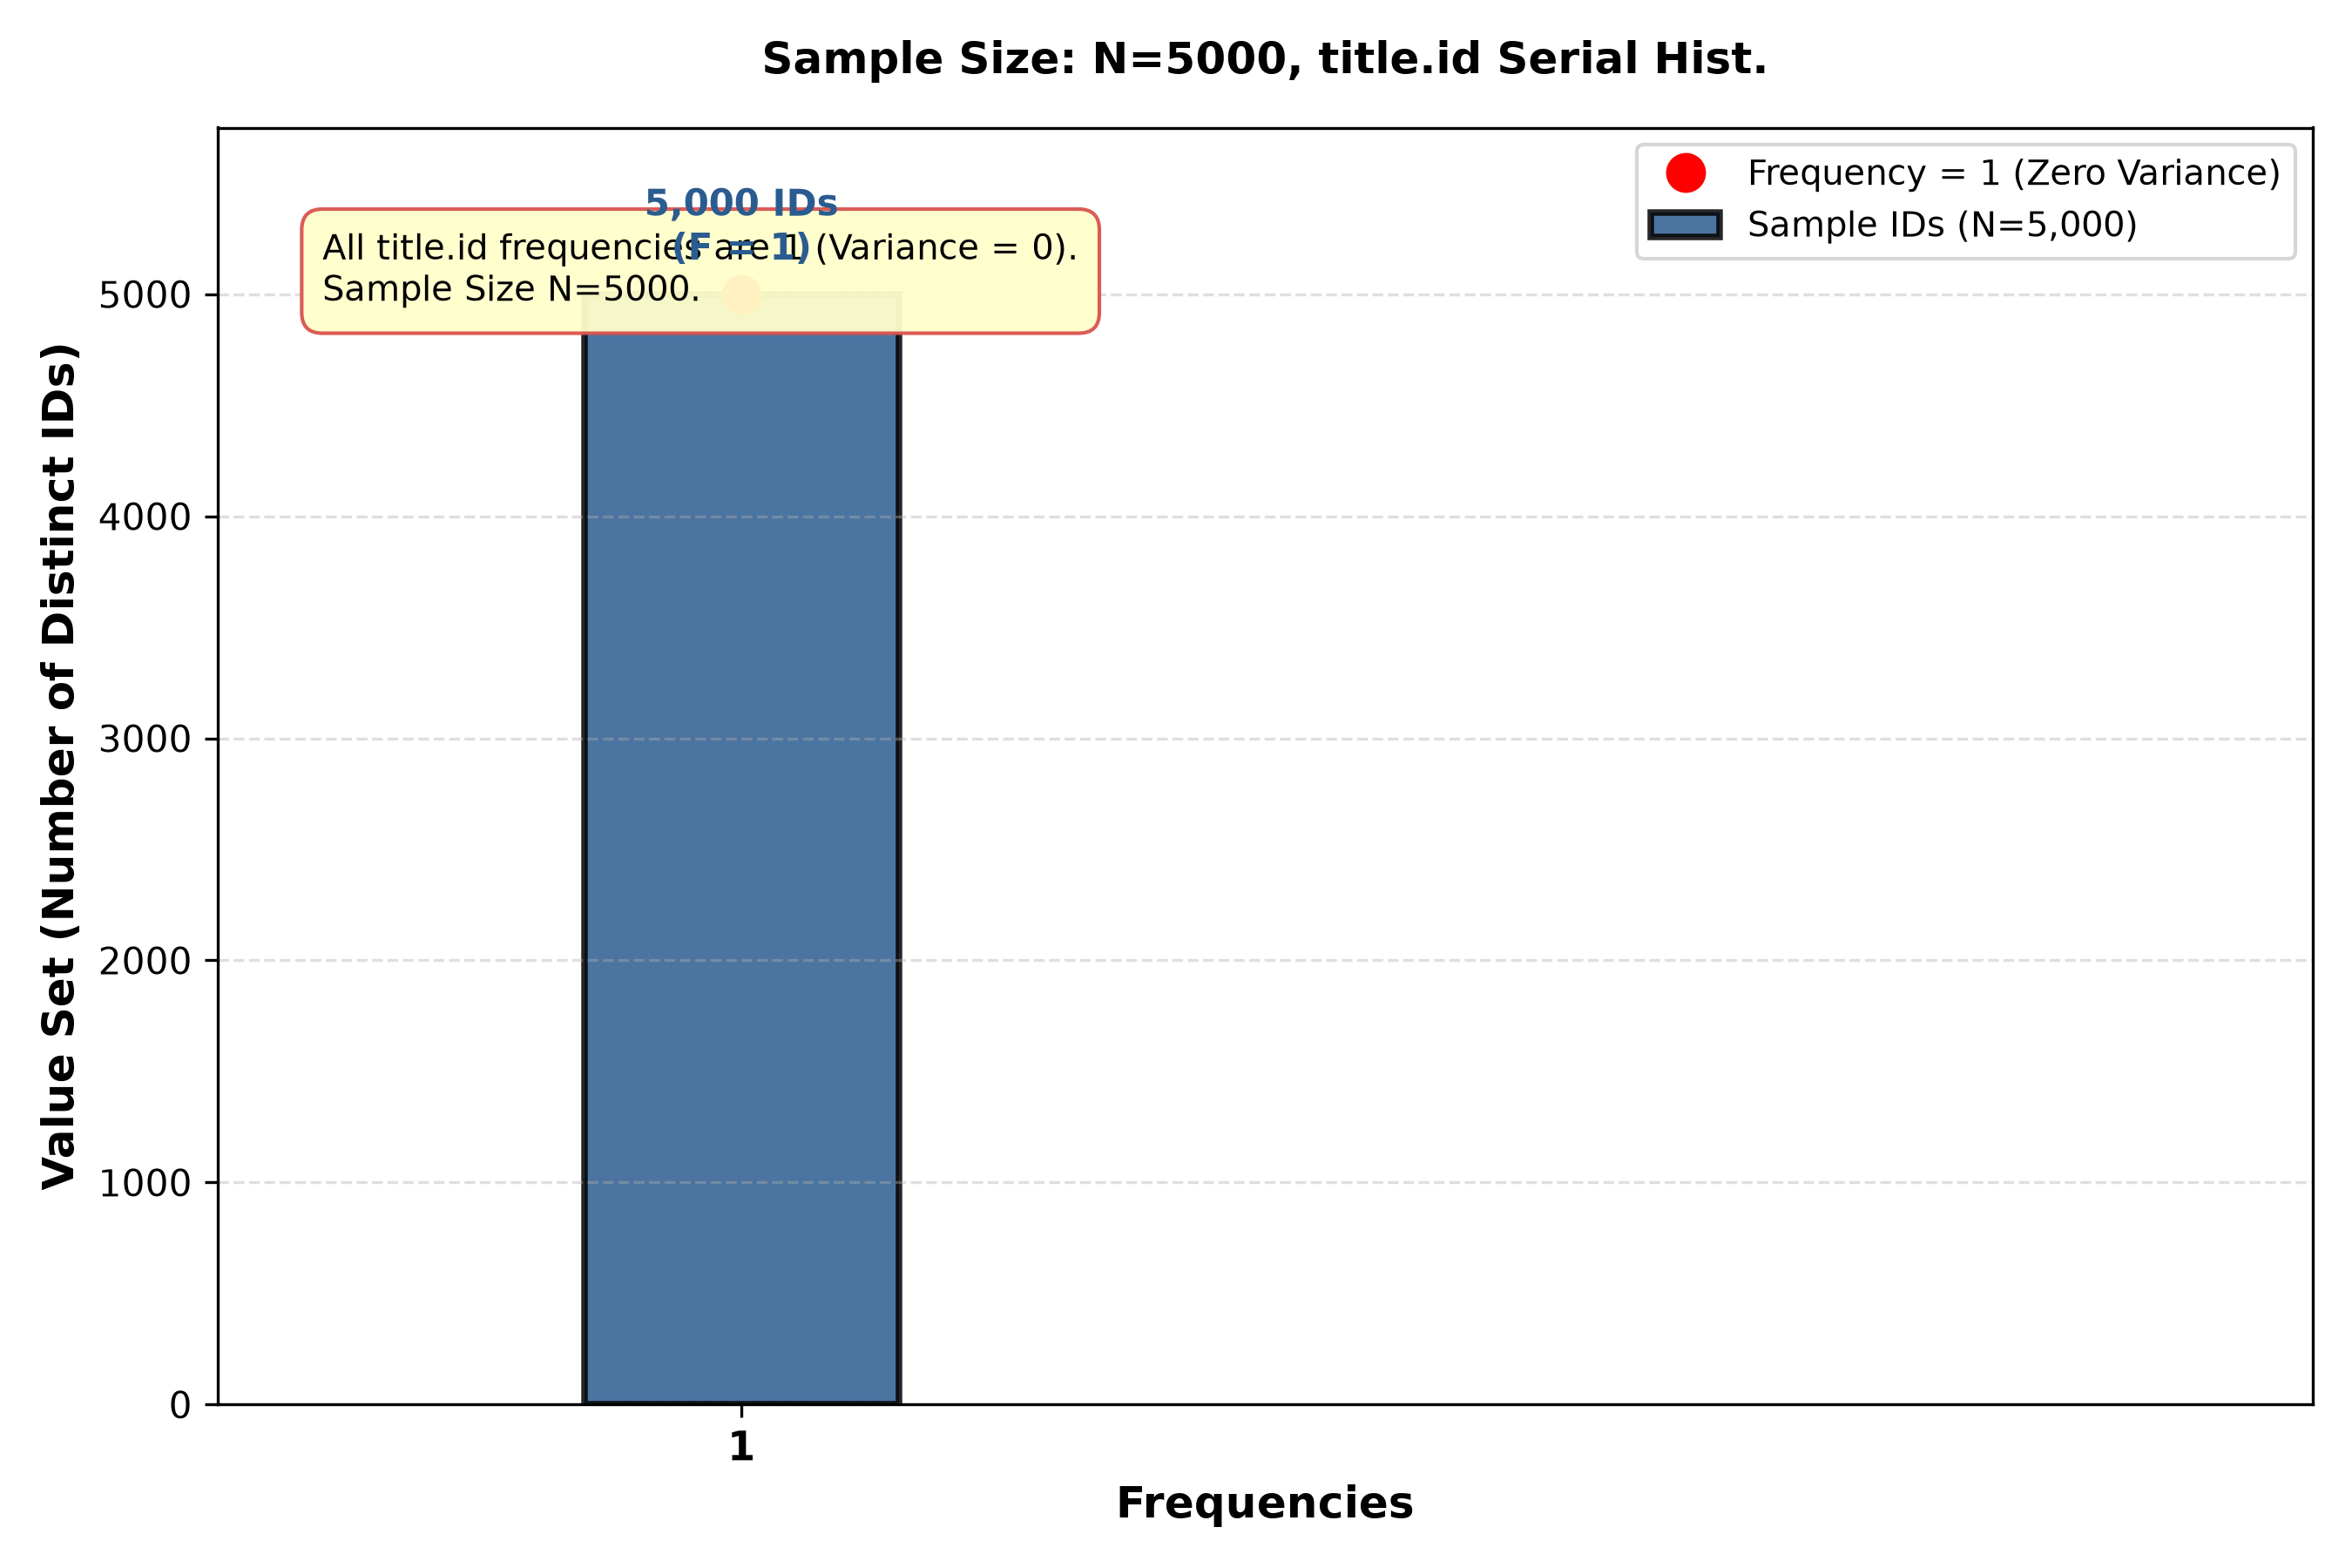
\includegraphics[width=0.85\textwidth]{q2_histogram_id_5000.png}
\caption{Sample Size: N=5000, title.id Serial Hist.}
\end{figure}

\begin{figure}[H]
\centering
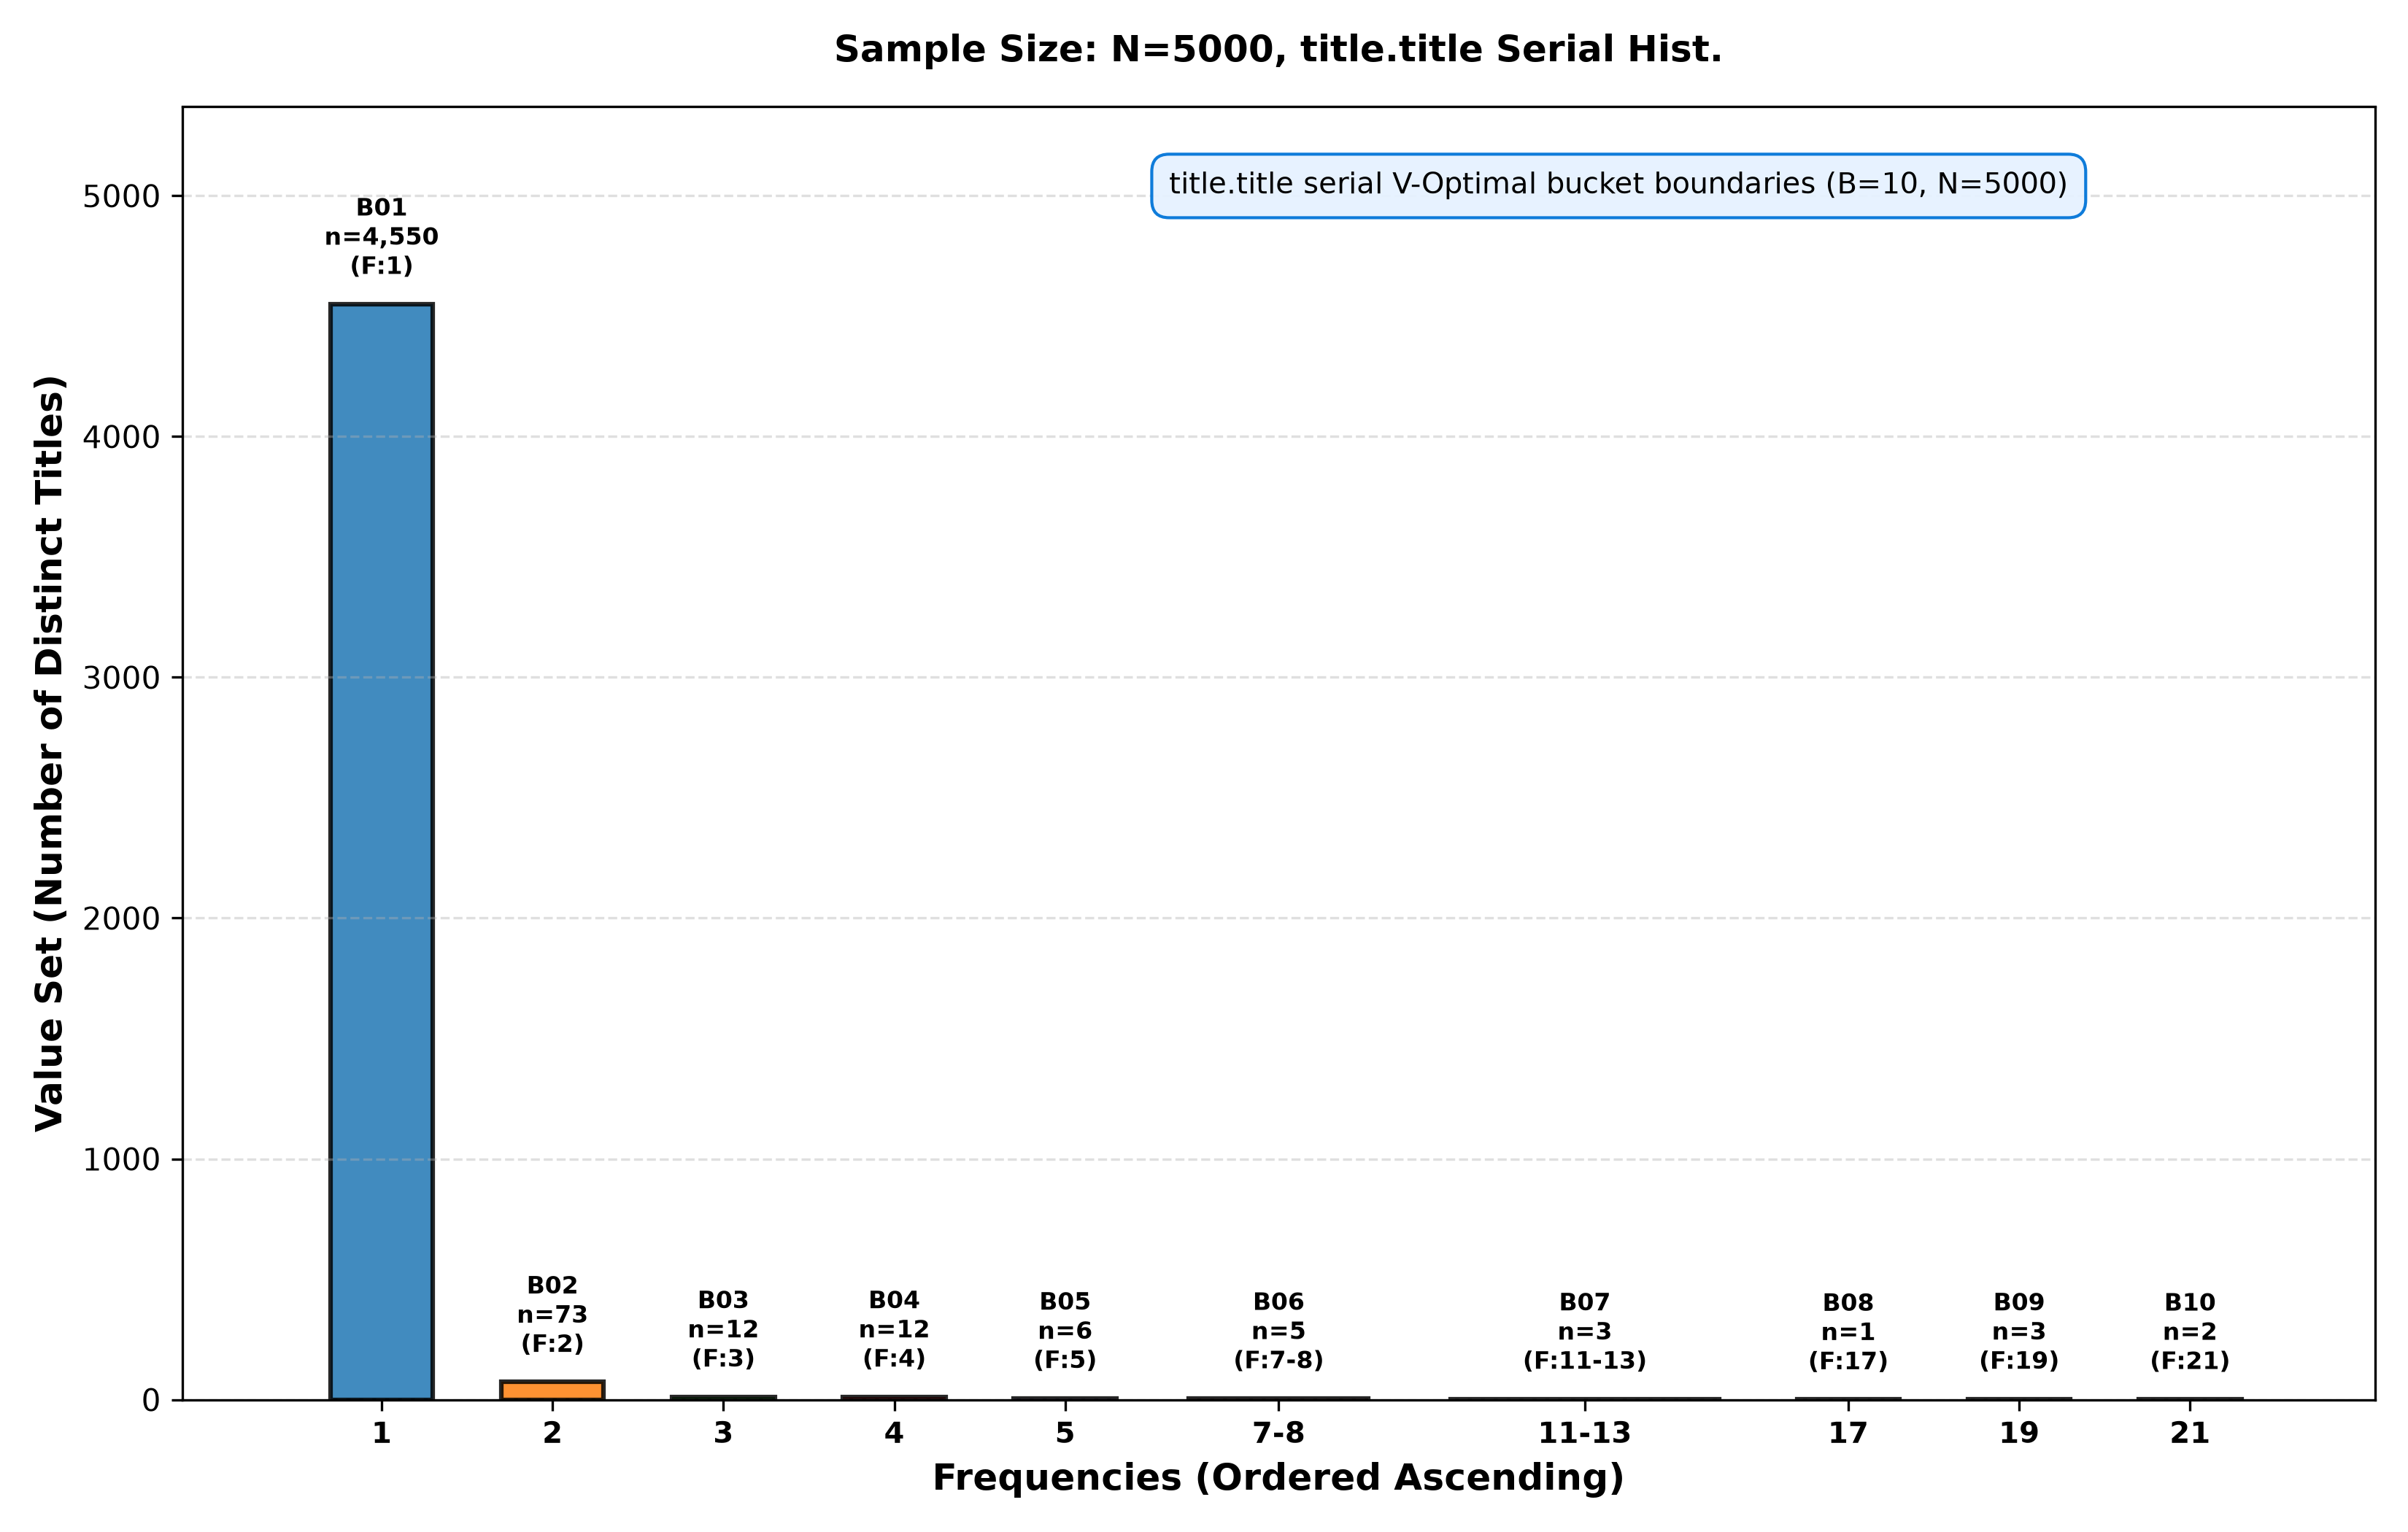
\includegraphics[width=0.85\textwidth]{q2_histogram_title_5000.png}
\caption{Sample Size: N=5000, title.title Serial Hist.}
\end{figure}

\paragraph{D. Comprehensive 3-Run Summary Table Across Exact Sample Sizes}
{\begingroup
\footnotesize
\setlength{\tabcolsep}{3.5pt}
\begin{xltabular}{\textwidth}{C | C | C | C | C | C | C}
\toprule
\textbf{Exact Sample Size ($N$)} & \textbf{Column} & \textbf{Run 1 Error} & \textbf{Run 2 Error} & \textbf{Run 3 Error} & \textbf{\textbf{Average Max Error}} & \textbf{Average Build Time} \\
\midrule
\endfirsthead
\toprule
\textbf{Exact Sample Size ($N$)} & \textbf{Column} & \textbf{Run 1 Error} & \textbf{Run 2 Error} & \textbf{Run 3 Error} & \textbf{\textbf{Average Max Error}} & \textbf{Average Build Time} \\
\midrule
\endfirsthead
\endhead
\bottomrule
\endfoot
\bottomrule
\endlastfoot
\textbf{1000} & \texttt{id} & \texttt{0.020667} & \texttt{0.013333} & \texttt{0.016556} & \textbf{\texttt{0.016852}} & \texttt{0.2370s} \\
\textbf{1000} & \texttt{title} & \texttt{0.637000} & \texttt{0.625000} & \texttt{0.169333} & \textbf{\texttt{0.477111}} & \texttt{0.3204s} \\
\textbf{3000} & \texttt{id} & \texttt{0.022444} & \texttt{0.009556} & \texttt{0.009889} & \textbf{\texttt{0.013963}} & \texttt{0.2118s} \\
\textbf{3000} & \texttt{title} & \texttt{0.612556} & \texttt{0.609000} & \texttt{0.616667} & \textbf{\texttt{0.612741}} & \texttt{0.3122s} \\
\textbf{5000} & \texttt{id} & \texttt{0.013578} & \texttt{0.005778} & \texttt{0.007556} & \textbf{\texttt{0.008970}} & \texttt{0.2394s} \\
\textbf{5000} & \texttt{title} & \texttt{0.603667} & \texttt{0.600667} & \texttt{0.606400} & \textbf{\texttt{0.603578}} & \texttt{0.3256s} \\
\end{xltabular}
\endgroup}


\hrule


\subsubsection{6. Full Step-by-Step Linear Regression Extrapolation ($N = 2,528,312$)}

To extrapolate the construction build time for the entire \texttt{title} table ($N = 2,528,312$), we fit a linear regression model on the 3-run average measured build times:

\[ T(N) = m \cdot N + c \]


\paragraph{A. Sample Data Points $(N_i, T_i)$}
\begin{itemize}
\item Point 1: $(N_1, T_1) = (1000, 0.2370)$
\item Point 2: $(N_2, T_2) = (3000, 0.2118)$
\item Point 3: $(N_3, T_3) = (5000, 0.2394)$
\end{itemize}

\paragraph{B. Mean Calculations}
\begin{itemize}
\item $\bar{N} = \frac{1000 + 3000 + 5000}{3} = \mathbf{3000}$
\item $\bar{T} = \frac{0.2370 + 0.2118 + 0.2394}{3} = \mathbf{0.2294\text{ seconds}}$
\end{itemize}

\paragraph{C. Deviations \& Sum of Products}
{\begingroup
\footnotesize
\setlength{\tabcolsep}{3.5pt}
\begin{xltabular}{\textwidth}{C | C | C | C | C | C}
\toprule
\textbf{$N_i$} & \textbf{$T_i$ (s)} & \textbf{$(N_i - \bar{N})$} & \textbf{$(T_i - \bar{T})$} & \textbf{$(N_i - \bar{N})^2$} & \textbf{$(N_i - \bar{N})(T_i - \bar{T})$} \\
\midrule
\endfirsthead
\toprule
\textbf{$N_i$} & \textbf{$T_i$ (s)} & \textbf{$(N_i - \bar{N})$} & \textbf{$(T_i - \bar{T})$} & \textbf{$(N_i - \bar{N})^2$} & \textbf{$(N_i - \bar{N})(T_i - \bar{T})$} \\
\midrule
\endfirsthead
\endhead
\bottomrule
\endfoot
\bottomrule
\endlastfoot
1000 & 0.2370 & -2000 & 0.0076 & 4,000,000 & -15.2143 \\
3000 & 0.2118 & 0 & -0.0176 & 0 & -0.0000 \\
5000 & 0.2394 & +2000 & 0.0100 & 4,000,000 & 20.0143 \\
\textbf{Sum} &  &  &  & \textbf{8,000,000} & \textbf{4.8000} \\
\end{xltabular}
\endgroup}


\paragraph{D. Slope ($m$) and Intercept ($c$) Formulas}
\begin{itemize}
\item **Slope ($m$)**:
\end{itemize}
\[ m = \frac{\sum (N_i - \bar{N})(T_i - \bar{T})}{\sum (N_i - \bar{N})^2} = \frac{4.8000}{8,000,000} = \mathbf{0.00000060\text{ seconds / sample}} \]


\begin{itemize}
\item **Intercept ($c$)**:
\end{itemize}
\[ c = \bar{T} - m \cdot \bar{N} = 0.2294 - (0.00000060 \times 3000) = \mathbf{0.227576\text{ seconds}} \]


\paragraph{E. Extrapolated Build Time for Full Table ($N = 2,528,312$)}
\[ T(2,528,312) = (0.00000060 \times 2,528,312) + (0.227576) = \mathbf{1.74\text{ seconds}} \quad (\mathbf{0.03\text{ minutes}}) \]


\hrule


\subsubsection{7. Sample Size vs Time Relationship Plot}
\begin{figure}[H]
\centering
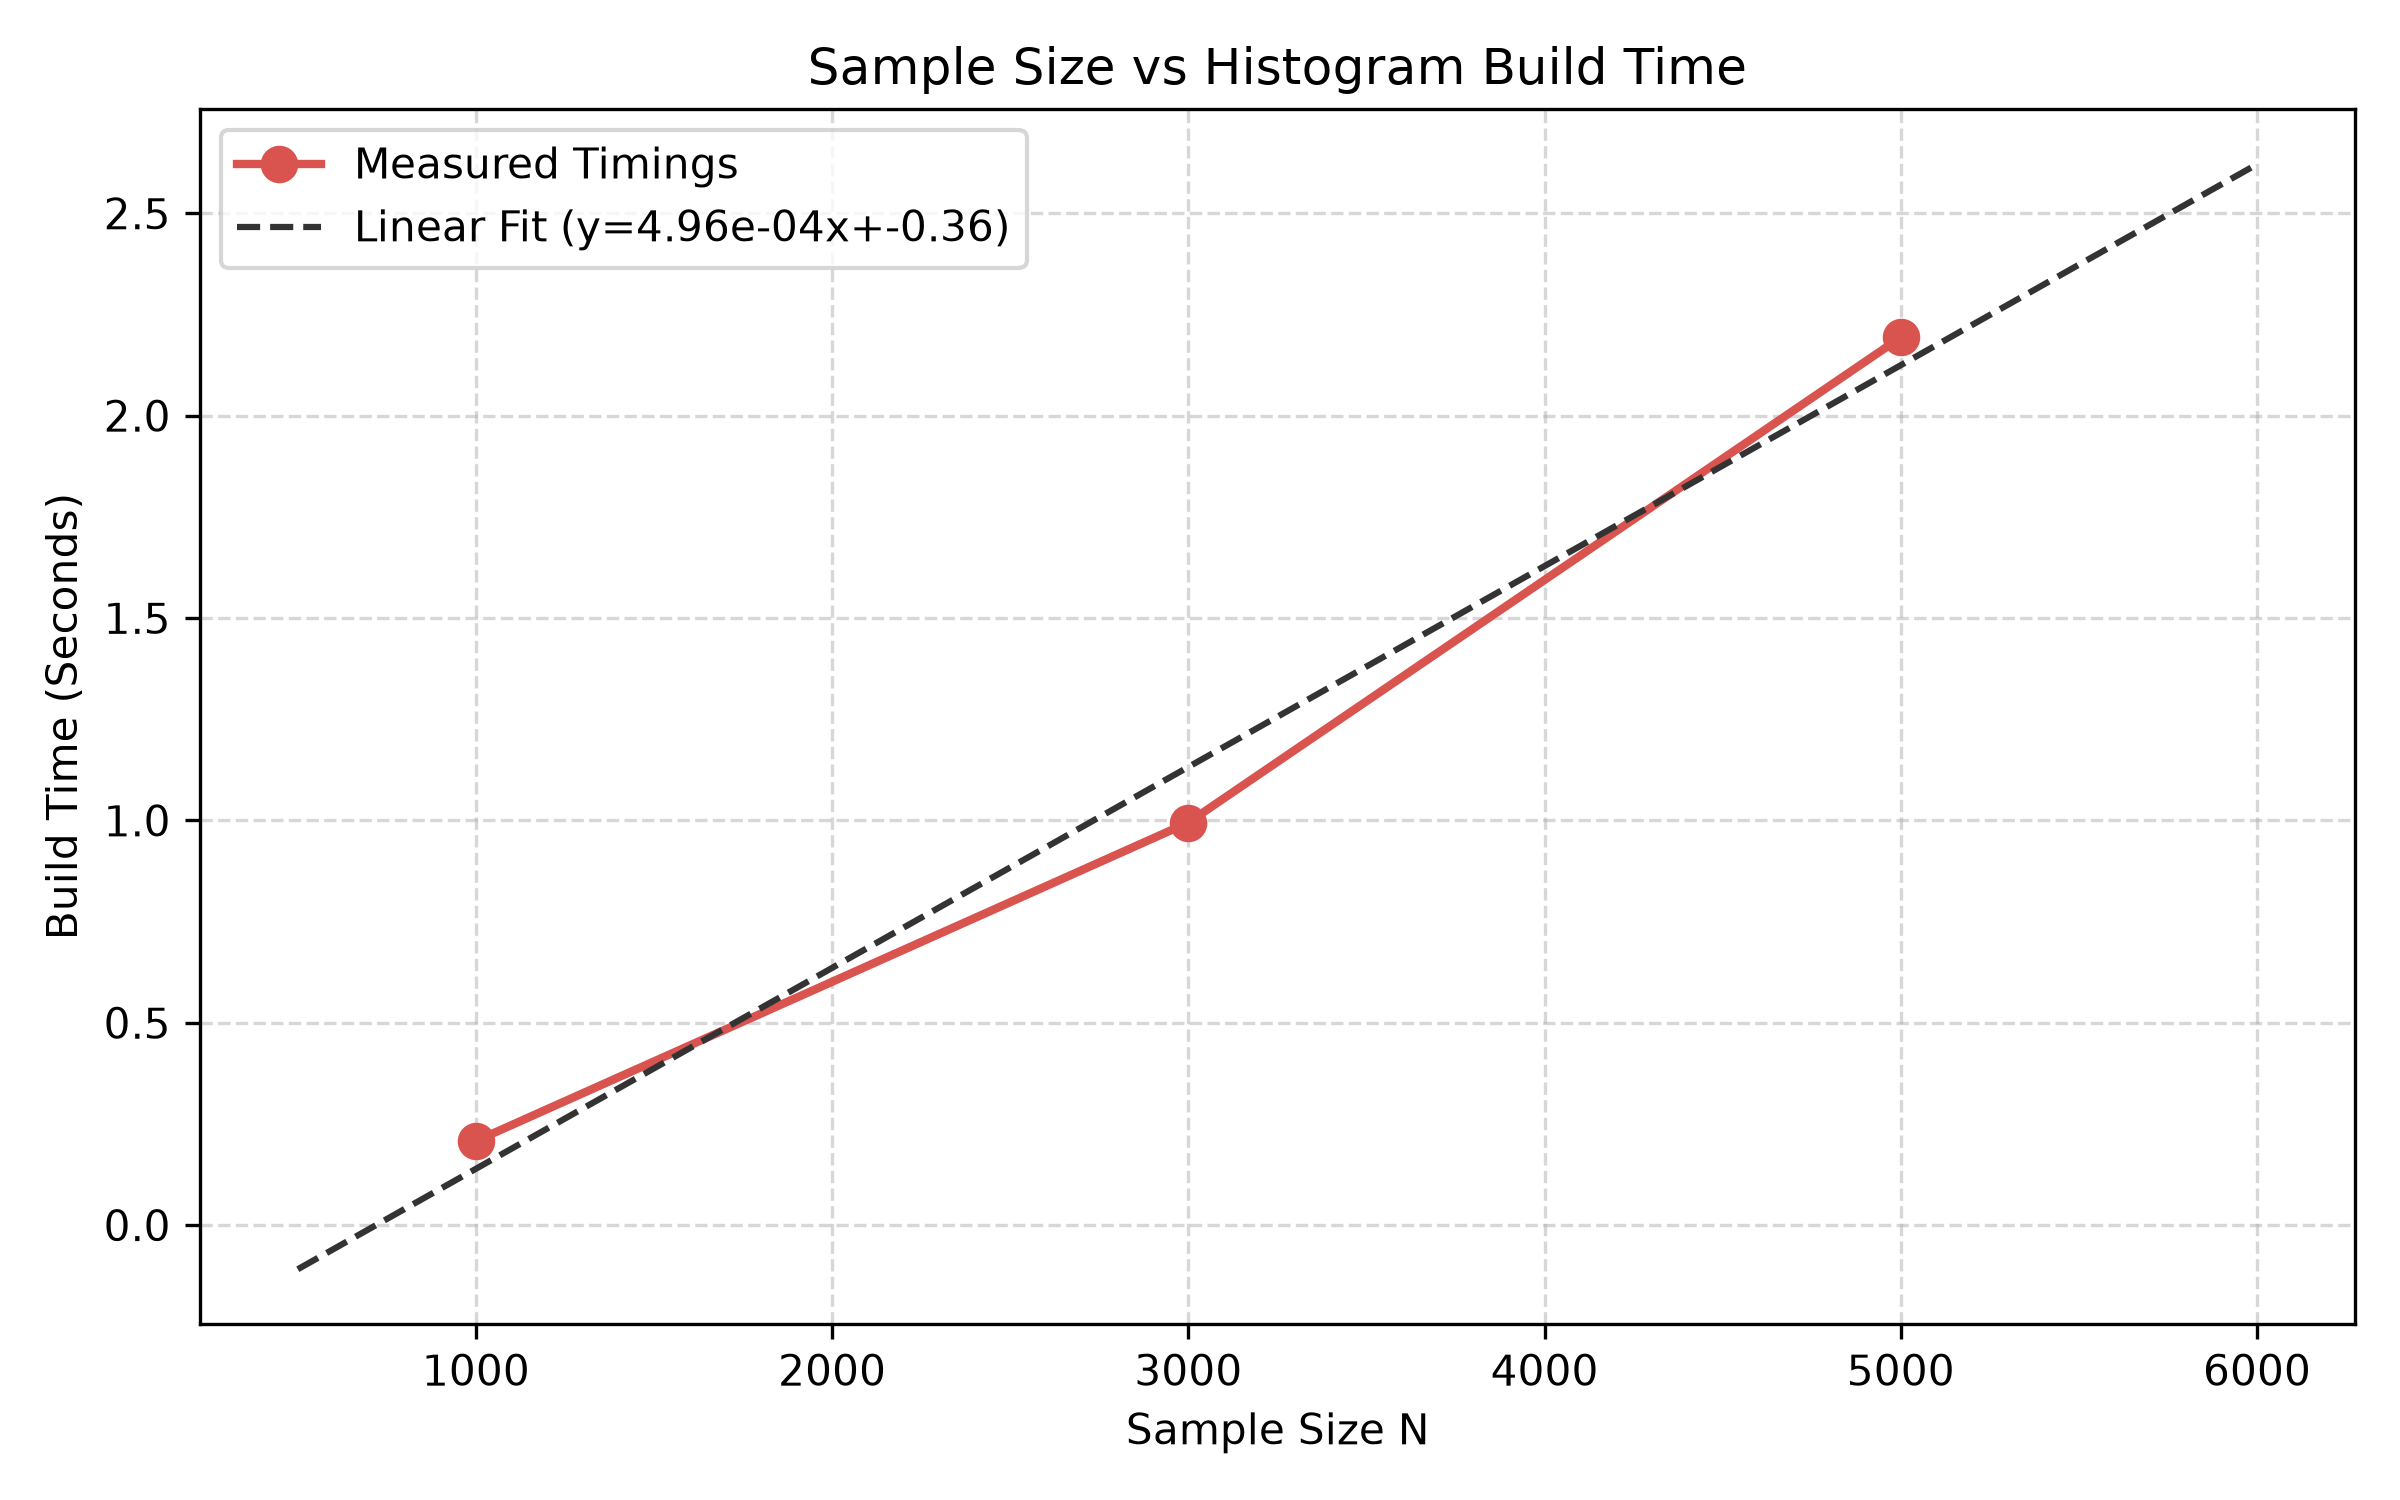
\includegraphics[width=0.85\textwidth]{q2_sample_size_vs_time.png}
\caption{Sample Size vs Time}
\end{figure}

\hrule


\subsubsection{8. Sample Size vs Max Selectivity Error Relationship Plot}
\begin{figure}[H]
\centering
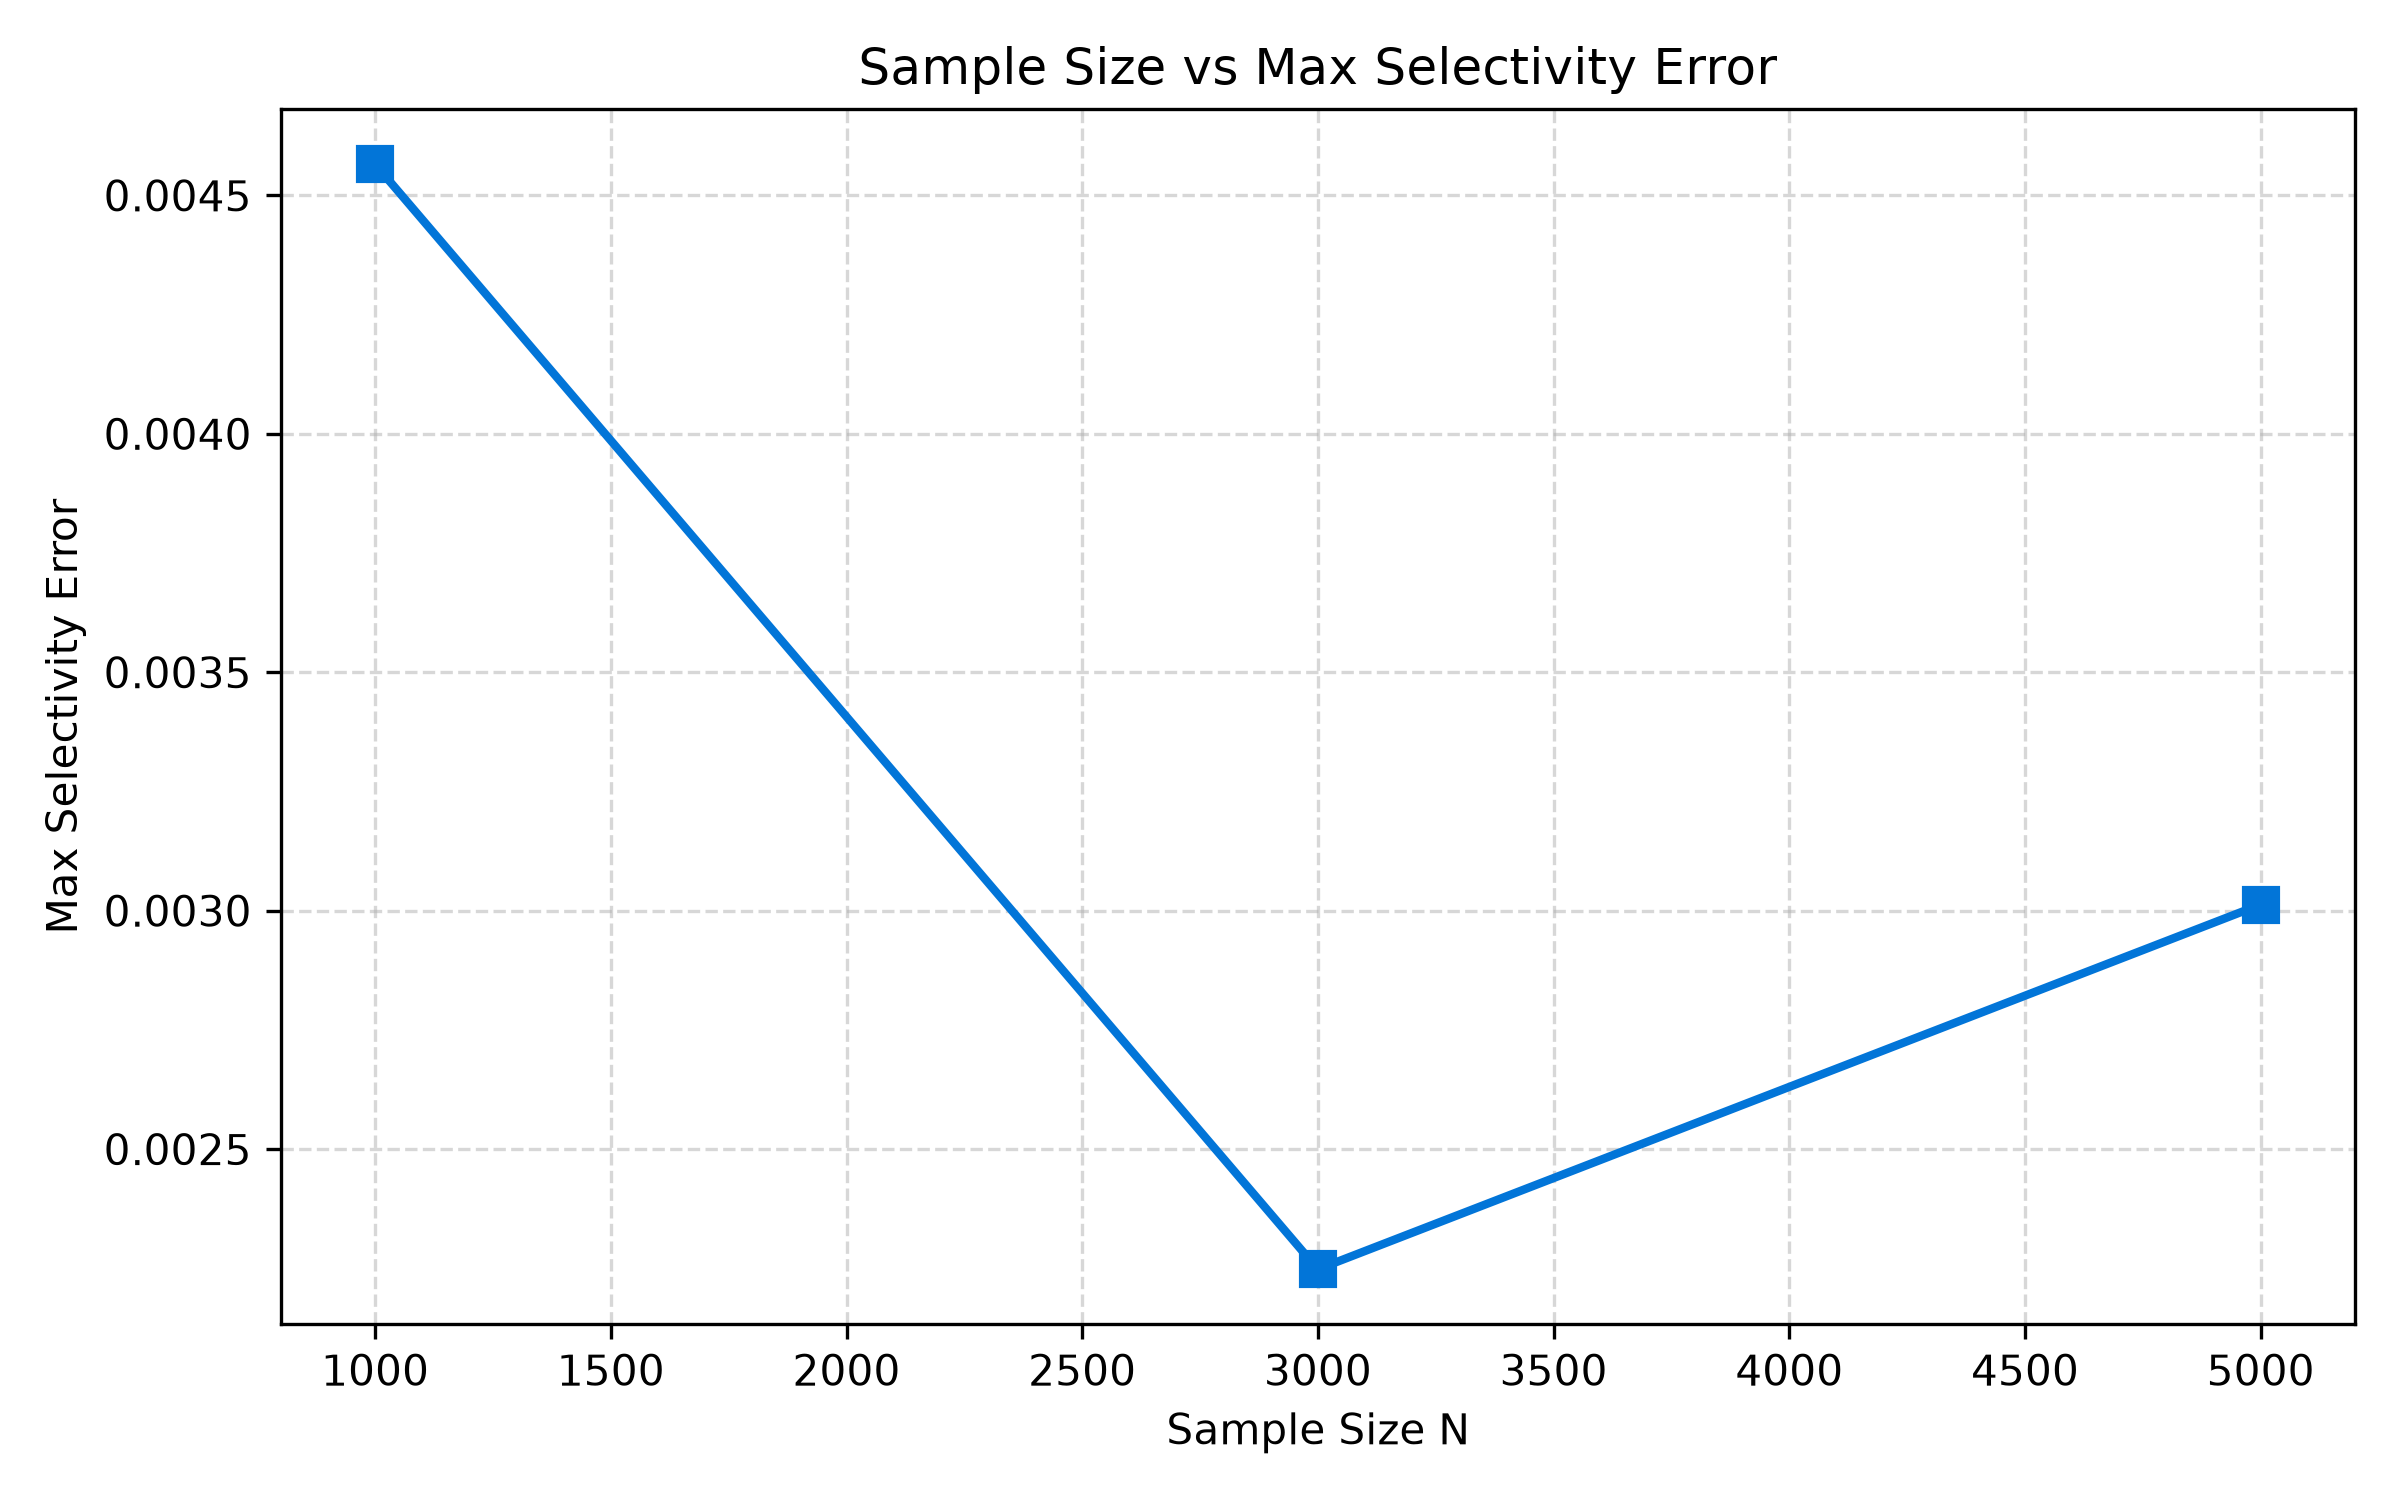
\includegraphics[width=0.85\textwidth]{q2_sample_size_vs_error.png}
\caption{Sample Size vs Max Selectivity Error}
\end{figure}

\hrule


\subsection{9: The Trade-off of Bucket Counts}

When building a histogram, choosing the number of buckets ($B$) is a classic trade off between performance and accuracy.


\textbf{Choosing Fewer Buckets (e.g., 5 to 10)}

If we use a small number of buckets, the biggest advantage is speed and efficiency. The histogram takes up very little memory in the system catalog and builds much faster because the time complexity of our algorithm, $O(B \cdot N^2)$, drops significantly. The query planner also spends less time analyzing it. However, the major downside is that we lose a lot of data resolution. Because the buckets are so wide, the internal mathematical estimates become much less accurate, especially if the data is heavily skewed or unevenly distributed.


\textbf{Choosing More Buckets (e.g., 50 to 100)}

On the flip side, using a large number of buckets gives the database a high-definition view of how the data is distributed. The estimates become incredibly precise, which leads to much lower selectivity errors and helps the query optimizer make smarter decisions for complex joins. The catch is that this accuracy comes at a heavy system cost. It takes noticeably longer to calculate and construct the histogram, consumes more storage space, and adds a slight delay to the query planning phase before execution can actually begin.

\end{document}
